\chapter{THE DARPA SC$2$ RADIO DESIGN}\label{B}
As discussed in Chapter \ref{A}, the ever-increasing demand for spectrum resources\texttt{-{}-}fueled by the massive MTC (IoT devices, VANs, WSNs), high-capacity user applications (UHD real-time video streaming, cloud-based applications, consumer device diversity), and advancements in military technologies\texttt{-{}-}has caused governments around the world to focus a lot of resources at scaling up, protecting, and maintaining the wireless communication infrastructure. In this regard, the DARPA Spectrum Collaboration Challenge (SC2) aims to bring in the enormous might of private industry, academic research organizations, and independent technology entrepreneurs to compete in a nation-wide competition that would result in the delivery of breakthrough technologies in the cognitive radio space\texttt{-{}-}particularly promoting the exploitation of advancements in collaborative A.I. and the plethora of capabilities offered by software-defined radios.

In this chapter, we discuss the design of the software-defined radio node developed by the Purdue BAM! Wireless team which competed in the DARPA SC2. The BAM! Wireless software-defined radio operates as either a Standard Radio Node (SRN)\texttt{-{}-}of which there are many in a given emulation scenario\texttt{-{}-}the primary responsibilities for which include:
\begin{itemize}
    \item Interacting with the DARPA SC2 emulation environment, i.e., the Colosseum, using the pre-determined and agreed-upon radio API,
    \item Delivering the assigned network flows within our network,
    \item Performing Power Spectral Density (PSD) measurements
    \item Following the various decisions made by the Gateway node in every layer of the protocol stack, and
    \item Sharing its PSD measurements, along with any other relevant metrics, with the Gateway node;
\end{itemize}
or a Gateway node\texttt{-{}-}of which there is just one deployed for our network in a given emulation scenario\texttt{-{}-}the primary responsibilities for which include:
\begin{itemize}
    \item Communicating with other competitor networks using the peer-reviewed and standardised Collaborative Intelligent Radio Network (CIRN) Interaction Language (CIL) over a dedicated collaboration channel,
    \item Coordinating channel access decisions, bandwidth allocation decisions, incumbent interference monitoring activities, and scoring analysis activities, among others.
\end{itemize}
In Section \ref{B.I} of this chapter, we discuss the various strategies employed in different layers of our radio's network protocol stack; in Section \ref{B.II}, we detail the radio API; in Section \ref{B.III}, we describe the CIRN Interface Language (CIL); in Section \ref{B.IV}, we present the performance results of various components of our radio operating in various military and disaster-relief scenarios; and finally, in Section \ref{B.V}, we present our concluding arguments.
\section{Cognitive Radio Subsystems}\label{B.I}
\subsection{Transmission Power Control (PHY)}\label{B.I.I}
In the ``Passive Incumbent Protect" SC2 scenario\texttt{-{}-}emulated in the Colosseum\texttt{-{}-}a licensed radio has prioritized access to the RF spectrum ($20$MHz bandwidth) and requires that the aggregate interference caused to its transmissions, in that bandwidth, by the radios of the competitors, should be below a specified threshold \cite{DARPA:SC2pi}. This threshold varies over time and varies based on the amounts of interference caused by the cognitive radio nodes, i.e., the threshold changes over time according to a pre-configured schedule and there are additional threshold tightening challenges wherein if the aggregate interference caused by the competitors exceeds the nominal threshold, the threshold becomes more stringent and will stay there until the aggregate interference drops below this stricter threshold\texttt{-{}-}additionally, the threshold will drop back to its nominal setting if the aggregate interference stays below the stricter threshold for a pre-determined duration. We incorporate transmission power control in our radio's design to specifically address the challenges brought on by this incumbent protection scenario. As a part of its design the Passive Incumbent, emulated in the Colosseum, performs periodic relative-power measurements in its specified $20$MHz RF spectrum of interest, compares these measurements with the current aggregate interference threshold setting, and broadcasts warning or violation messages to the competitors over the collaboration network.

When the relative-power spectrum measurements at the Passive Incumbent exceed its current threshold, and this persists for a pre-defined duration, the Passive Incumbent broadcasts a ``Violation" message to the competitors over the collaboration network. Upon receiving this violation message, the transmission power at every SRN within each competitor network should be lowered (collaboratively) until the aggregate interference level at the Passive Incumbent drops below the threshold. The competitor networks can also rely on the Passive Incumbent's ``Report" messages to determine if the SRN transmit power has to be lowered in anticipation of exceeding the allowed interference at the Passive Incumbent.

Now, specifically focusing on the transmission power control strategy at the SRNs in our network, deployed in a Passive Incumbent SC2 scenario: based on the CIL messages received from other competitor networks and knowing the occupancy characteristics of the SRNs in our network, our decision engine first determines the number of radio nodes in this deployment that are accessing portions of the spectrum under observation or under use by the Passive Incumbent, denoted by $\Lambda$, i.e., all the radios in all the competitor networks participating in this scenario that are occupying fragments of the $20$MHz spectrum under observation by the Passive Incumbent\texttt{-{}-}including our own\texttt{-{}-}we reduce the transmission power of our SRNs by a factor proportional to the difference between the aggregate interference power measured by the Passive Incumbent and its current threshold setting, divided by $\Lambda$, i.e., 
\begin{equation}\label{B.1}
    P_{T}'=P_{T}-\left(\frac{P_{obs}-\omega P_{th}}{\Lambda}\right),
\end{equation}
where $P_{T}$ denotes the transmit power of SRNs in our network (in dBFS), 
\begin{equation}\label{B.2}
    P_{obs}=10\log_{10}(I^{2}{+}Q^{2})-31.5\text{\cite{DARPA:SC2pi},}
\end{equation}
denotes the relative-power measured at the Passive Incumbent (in dBFS), $P_{th}$ denotes the current threshold of the Passive Incumbent (in dBFS), and $\omega$ (slightly less than $1$) is a multiplicative offset factor to account for synchronization inconsistencies. Here, for this formulation to work successfully and result in the aggregate interference observed at the Passive Incumbent to be
\begin{equation}\label{B.3}
    P_{obs}=\sum_{\nu}\sum_{\mu}(P_{T}')^{\nu,\mu}=\sum_{\lambda=1}^{\Lambda}\left(P_{T}-\frac{\Lambda P_{T}}{\Lambda}+\frac{{\omega}P_{th}}{\Lambda}\right)={\omega}P_{th}<P_{th},    
\end{equation}
where $\nu$ represents the competitor index, $\mu$ represents the SRN index within a given competitor network\texttt{-{}-}we ensure that all competitors make similar adjustments in the transmit power of their respective SRNs, by collaborating with them via CIL messages over the collaboration network.
\subsection{Network Control Data Broadcast}\label{B.I.II}
There are two types of network control messages employed in our radio. The first being the so-called ``short" control message that is transmitted using a non-coherent $8$-FSK modulated link using a channel of $480$kHz bandwidth and whose center frequency changes every second between the upper and lower band edges of the RF spectrum determined by the Colosseum environment; with Reed-Solomon error control coding; and a time-hopping synchronization technique. Every SRN broadcasts these short control messages to all the other SRNs in our network, and these messages contain information regarding the number of SRNs in our network, the current channel allocation of this SRN, and a timestamp. This FSK control channel uses the following media access scheme: Considering a slot duration of $60$ms, at the beginning of each time-slot, each SRN in our network transmits its short control message packet over the FSK control channel with a probability of $\frac{1}{\tilde{\Lambda}}$, where $\tilde{\Lambda}$ denotes the number of SRNs in our network\texttt{-{}-}additionally, packet collisions that occur between/among concurrent short control message transmissions of two or more SRNs result in decoding errors, and are hence discarded at the receiver. When an SRN receives a short control message from another SRN in our network, it updates its view of the network, and re-broadcasts this modified ``observed network state" to other SRNs in the network. The short control messages are primarily used for network bootstrapping and for the node discovery phase during network setup. Additionally, this FSK control channel serves as a fallback mechanism for all control data in high-interference communication environments. 
\begin{figure} [htb]
    \centerline{
    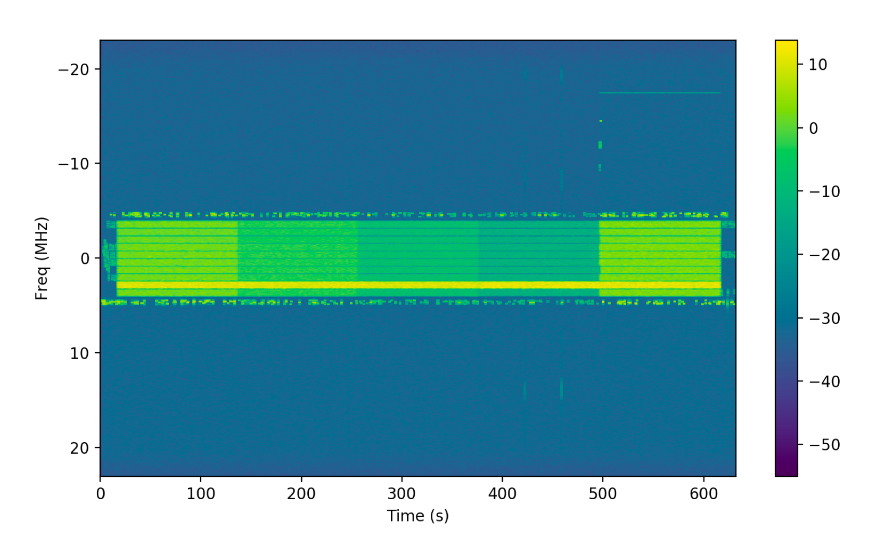
\includegraphics[width = 1.0\textwidth]{Control_Channels_At_Band_Edges.PNG}}
    \caption{The power spectrum observed by an SRN during an SC2 qualification run}
    \label{fig:B.1}
\end{figure}

The second type of control message, i.e., the ``long" control message, contains information regarding traffic statistics, QoS metrics relevant for scoring (SC2 scoring ``rates" the performance of our network as a whole, by assigning points to successfully completed delivery of assigned flows at each source-destination pair in our network), the estimated noise-variance matrix, and DLL flow schedule updates, among others. Each SRN in our network broadcasts these long control messages every second, interleaved with the data traffic\texttt{-{}-}transmitted over the DFT-s-OFDM high data rate link (discussed in \ref{B.I.III}) using the center frequency and bandwidth assigned to this SRN by the Gateway SRNs current channel allocation strategy. Fig. \ref{fig:B.1} illustrates the fact that ``short" control transmissions employ the upper and lower band-edges of the spectrum, while ``long" control transmissions are interleaved with data and sent over the four wideband channels.
\subsection{The DFT-s-OFDM Data Link}\label{B.I.III}
As outlined in Section \ref{B.I.II}, both data traffic and ``long" control message traffic are transmitted by the SRNs in our network over the high data rate Discrete Fourier Transform-spread-Orthogonal Frequency Division Multiplexing (DFT-s-OFDM) channel\texttt{-{}-}using the center frequency and bandwidth assigned to the corresponding SRN, according to the current channel access action determined by the Gateway SRN. Each SRN, upon receiving the current channel and bandwidth allocations for all the other $\tilde{\Lambda}{-}1$ SRNs in our network\texttt{-{}-}over the FSK control link (i.e., ``short" control messages) described in Section \ref{B.I.II}\texttt{-{}-}tunes its $\tilde{\Lambda}{-}1$ receive chains to these $\tilde{\Lambda}{-}1$ channels (center frequency and bandwidth information shared by the other SRNs over the FSK control link), and is therefore able to receive transmissions from all the other SRNs in our network. Additionally, these receive chains perform Schmidl \& Cox time synchronization and frequency offset compensation, in addition to channel noise variance estimation and frequency-domain equalization. All waveforms in this high data rate link constitute $128$ sub-carriers: $108$ are used for data symbols, $12$ are used for pilot symbols, and the remaining $8$ are used for null transmissions that are essential for channel noise variance estimation (the estimates are used in the MCS adaptation technique described in Section \ref{B.I.IV}).
\begin{figure} [htb]
    \centerline{
    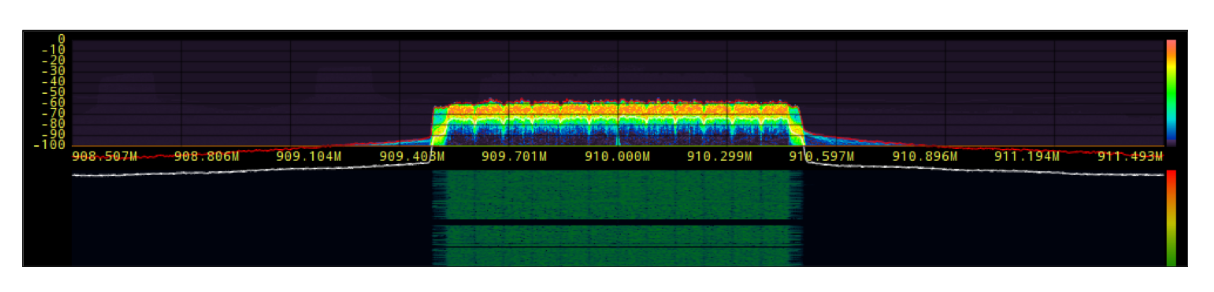
\includegraphics[width = 1.0\textwidth]{Data_Channel_DFT-spread-OFDM_Power_Spectrum.PNG}}
    \caption{The power spectrum of the DFT-s-OFDM waveform}
    \label{fig:B.2}
\end{figure}

A segment, which is the simplest data unit in the Data Link Layer (DLL) of our radio, can an IPv$4$ segment carrying Colosseum data or an IPv$4$ segment carrying ARQ data or a control segment. These segments in the DLL constitute the payload in a frame, which is the simplest data unit in the PHY. A PHY frame consists of a frame header\texttt{-{}-}which contains the source SRN ID, the destination SRN ID, the modulation order and code rate (MCS-$(\mathcal{M},\mathcal{R})$ pair discussed in Section \ref{B.I.IV}) used for the frame payload, a unique identifier for logging, a $32$-bit Cyclic Redundancy Check (CRC), and the number of code-words (blocks) in the frame payload\texttt{-{}-}with the frame header being modulated using QPSK and coded using a rate-$\frac{1}{2}$ Low Density Parity Check (LDPC) code; and the frame payload\texttt{-{}-}which constitutes a sequence of code-words (blocks) populated from a sequence of DLL segments\texttt{-{}-}with this frame payload being modulated and IEEE 802.11 Quasi-Cyclic LDPC (QC-LDPC) coded using an aptly chosen modulation order and code rate (MCS-$(\mathcal{M},\mathcal{R})$ pair discussed in Section \ref{B.I.IV}) which is additionally heralded in the frame header, and finally, mapped onto the sub-carriers of a sequence of OFDM symbols. It is important to note here that, as also discussed in Section \ref{B.I.IV}, the modulation schemes used in our design are QPSK ($\mathcal{M}{=}4$), QAM$16$ ($\mathcal{M}{=}16$), QAM$32$ ($\mathcal{M}{=}32$), and QAM$64$ ($\mathcal{M}{=}64$)\texttt{-{}-}and the code rates ($\mathcal{R}$) used in our design are $\frac{1}{2},\frac{2}{3},\frac{3}{4},\text{ and }\frac{5}{6}$. The power spectrum of the DFT-s-OFDM waveform is illustrated in Fig. \ref{fig:B.2}.
\subsection{Modulation and Coding Scheme (MCS) Adaptation (PHY)}\label{B.I.IV}
The MCS adaptation formulation used in the PHY is a link throughput maximization problem, performed at each individual link $l$ (i.e., a source-destination pair) in our network, subject to constraints on the minimum achieved throughput and maximum allowable bit error probability. This optimization problem involves maximizing the link throughput by finding the modulation order (${=}4,16,32,64$\texttt{-{}-}corresponding to QPSK, QAM$16$, QAM$32$, and QAM$64$, respectively), denoted by $\mathcal{M}$, and the code rate (${=}\frac{1}{2},\frac{2}{3},\frac{3}{4},\frac{5}{6}$), denoted by $\mathcal{R}$, having the smallest Euclidean distance between two circles centered about adjacent symbols in the constellation diagram, with the radius of each of these circles being proportional to the ratio of the estimated standard deviation of the additive channel noise (and the interference from other SRNs on this channel) to the asymptotic code gain. Additionally, in order to remove noise variance measurements with low probabilities of occurrence, we apply a sliding window median filter to the estimated noise variance. Furthermore, as a part of the constraint on the maximum allowable bit error probability, we employ a closed-form approximation for evaluating the bit error probability, denoted by $\mathbb{P}_{b}^{(l)}$, as a function of the noise variance estimate $\hat{\sigma}^{2}$ and the minimum constellation distance $d_{\text{min}}$, given by
\begin{equation}\label{B.4}
    \begin{cases}
        \mathbb{P}_{b}^{(l)}=Q\left(\frac{d_{\text{min}}}{\sqrt{2\hat{\sigma}^{2}}}\right),&\text{ if $\mathcal{M}=4$},\\
        \mathbb{P}_{b}^{(l)}=\frac{4}{\log_{2}(\mathcal{M})}Q\left(\frac{d_{\text{min}}}{\sqrt{2\hat{\sigma}^{2}}}\right),&\text{ if $\mathcal{M}>4$},
    \end{cases}
\end{equation}
where,
\begin{equation}\label{B.5}
    Q(x)=\frac{1}{2\pi}\int_{x}^{\infty}e^{-\frac{y^{2}}{2}}.
\end{equation}
The throughput over this link $l$, denoted by $\rho_{l}$, is given by
\begin{equation}\label{B.6}
    \rho_{l}=\mathcal{R} \cdot BW_{l} \cdot \log_{2}(\mathcal{M}),
\end{equation}
where $BW_{l}$ refers to the bandwidth allocated by the Gateway SRN for this link (based on PSD measurements and collaboration network messages, as a part of the channel access strategy in the MAC).
\begin{figure} [htb]
    \centerline{
    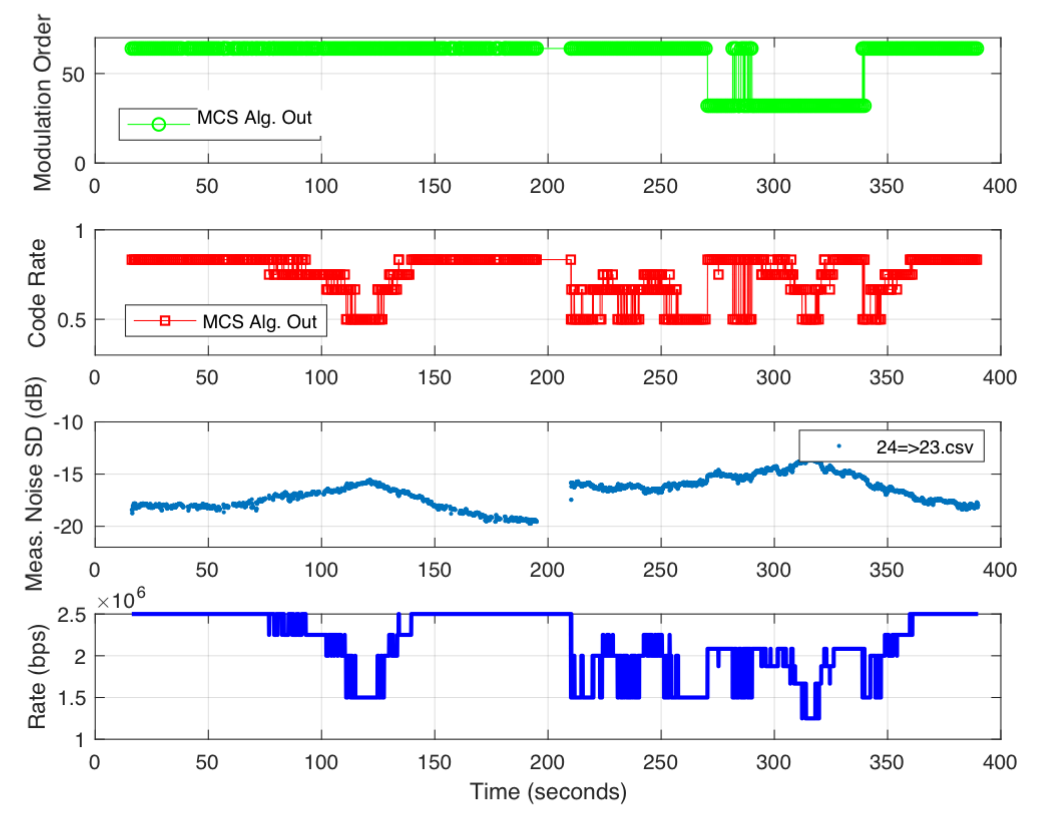
\includegraphics[width = 1.0\textwidth]{Payline_MCS_Adaptation.PNG}}
    \caption{The MCS adaptation scheme during a Payline scenario}
    \label{fig:B.3}
\end{figure}
\begin{figure} [htb]
    \centerline{
    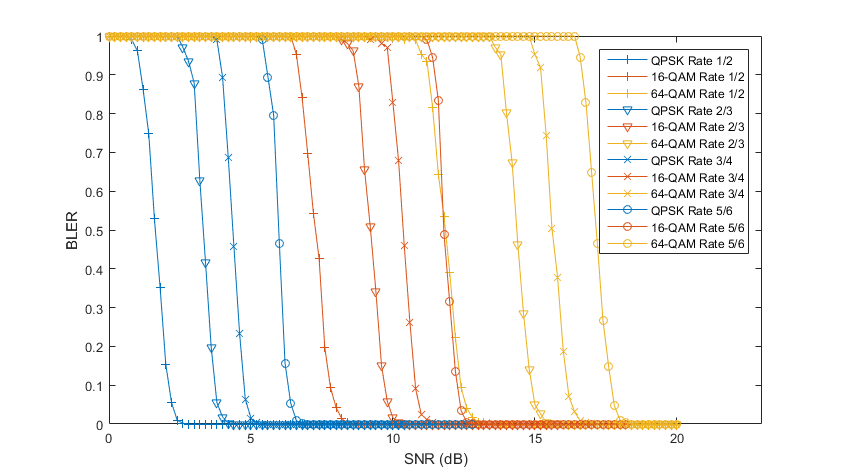
\includegraphics[width = 1.0\textwidth]{BLER.PNG}}
    \caption{The block error rates (BLERs) for different modulation order and code rate pairs, over varying values of SNR (dB)}
    \label{fig:B.4}
\end{figure}

So, at each link (source SRN-destination SRN), upon receiving a NotificationEvent (an inter-module memo in the C${++}$ publish-subscribe software architecture) which indicates a change in the estimated noise variance of the channel used by this link, the MCS adaptation algorithm involves finding the $(\mathcal{M},\mathcal{R})$ pair that has the smallest Euclidean distance between two circles centered about adjacent constellation points, with the radius of each circle given by the ratio of the current estimate of the standard deviation of the channel noise (and the interference caused by other SRNs on this channel) to the asymptotic code gain; subject to minimum required throughput and maximum allowable bit error probability requirements, i.e.,
\begin{equation}\label{B.7}
    \begin{aligned}
        &\min_{\mathcal{M},\mathcal{R}}\ d_{\text{min}}(\mathcal{M},\mathcal{R},\hat{\sigma}),\\
        &\text{subject to}\\
        &\rho_{l} \geq \rho_{l,\text{min}},\text{ and}\\
        &\mathbb{P}_{b}^{(l)} \leq \mathbb{P}_{b}^{(l,\text{max})},
    \end{aligned}
\end{equation}
where $\rho_{l,\text{min}}$ refers to the QoS constraint of supporting a minimum required throughput, $\mathbb{P}_{b}^{(l,\text{max})}$ refers to the maximum allowable bit error probability, $\mathbb{P}_{b}^{(l)}$ is computed using \eqref{B.5}, and $\rho_{l}$ is computed using \eqref{B.6}. Note here that a channel allocation update triggered by the Gateway SRN in our network, induces changes in the estimated (and filtered) noise variance map, which in turn triggers MCS adaptation. Consequently, MCS adaptation triggers an update to the flow schedule in the DLL, which is discussed in Section \ref{B.I.V}. Fig. \ref{fig:B.3} depicts the process of determining the most appropriate modulation order and coding rate adaptive to the changes in the estimated additive channel noise standard deviation. Note here that the link data rate reduces as the channel noise variance increases. Fig \ref{fig:B.4} illustrates the BLock Error Rate (BLER) curves for different combinations of the modulation order and the code rate, over different SNR values.
\subsection{Prioritized Flow Scheduling with ARQ Heuristic (DLL)}\label{B.I.V}
The prioritized flow scheduling algorithm employed in the DLL of our radio involves an adaptive time-quanta based deficit round-robin scheduler with a value-per-resource heuristic and recursive revisitation, in addition to Automatic Repeat reQuest (ARQ) for bursty User Datagram Protocol (UDP) flows (i.e., emulated file transfers). A DARPA SC2 emulation scenario in the Colosseum involves ``mandates" to deliver a variety of flows with pre-specified priorities\texttt{-{}-}quantified by their associated point-values. For instance, Voice Over Internet Protocol (VOIP) traffic is assigned 4 points per flow, the real-time camera feed from an Unmanned Aerial Vehicle (UAV) is assigned 9 points per flow, and the real-time continuous video stream from a water-bomber deployed to fight wildfires in California (emulated scenario) is assigned 15 points per flow. Additionally, a DARPA SC2 scenario also specifically categorizes flows into two groups: intermittent, bursty flows (file transfers) and all other non-bursty traffic.

Based on the available spectrum resources, i.e., channel bandwidth, and the amount of time remaining to complete an assigned flow, each flow is assigned time-quanta\texttt{-{}-}with a non-zero time-quanta assigned to a flow only if it is determined to be likely successful with the given time-quanta. The underlying infrastructure of our scheduler involves individual flow-specific at each SRN in our network\texttt{-{}-}additionally, this includes queues for file bursts and queues for ARQ packets that are supposed to be re-sent to the destination. At each SRN, we employ an ordered resource-fitting heuristic with recursive revisitation wherein we first determine the upper and lower bounds of the resource-block (which termed as a QuantumSchedule)\texttt{-{}-}where the lower bound represents the smallest amount of time required to send a frame corresponding to all the flow-queues at this SRN, subject to the quality of the links; while the upper bound represents the smallest maximum allowable latency among all the flows at this SRN, indicating a temporal resource bound at which ``mandates" start to fail. After determining the upper and lower bounds, based on its assigned flow metrics and quality of its links\texttt{-{}-}each SRN ranks (in decreasing order of priority) its assigned flows according a value-per-resource heuristic, determines the percentage utilization of the QuantumSchedule block for each of these flows (i.e.,  the resource block with the quantified upper and lower bounds), and starts fitting these flows onto the resource block with the added optimization of minimizing the amount of unused resources in this QuantumSchedule block\texttt{-{}-}a recursive revisitation strategy helps the scheduler to recursively perform an ordered fit routine on flows that are yet to be fitted onto the resource block with the intention of completely utilizing the QuantumSchedule block.

In more detail, as and when a new flow is assigned to a particular SRN $i$ in our network, the DLL creates a queue that holds the packets arriving at this SRN from the C2API (discussed in Section \ref{B.II}). When a schedule update is triggered by the arrival of new flows at the SRN, or when the channel and bandwidth allocation changes (as notified by the Gateway SRN via OFDMChannelUpdate NotificationEvents), or when the modulation order and code rate pair changes as a result of the MCS adaptation strategy in the PHY of this SRN (notified internally via MCSRequest NotificationEvents)\texttt{-{}-}the scheduler evaluates the smallest amount of temporal resources needed to serve each flow (on a frame-by-frame basis), i.e.,
\begin{equation}\label{B.8}
    t_{\text{min}}^{(f)}=\frac{f_{\text{ov}}+f_{\text{nseg}}(f_{\text{seg-ov}}+f_{\text{seg-bits}})}{\rho_{l_{f}}},
\end{equation}
where $f_{\text{ov}}$ refers to the frame overhead of flow $f$, $f_{\text{nseg}}$ refers to the number of DLL segments per frame of flow $f$, $f_{\text{seg-ov}}$ denotes a per segment overhead per frame of flow $f$, $f_{\text{seg-bits}}$ is the number of bits per segment of flow $f$, and $\rho_{l_{f}}$ indicates the link throughput\texttt{-{}-}evaluated using the allocated channel bandwidth, the estimated channel noise variance (and interference from competitor SRNs), and the $(\mathcal{M},\mathcal{R})$ pair\texttt{-{}-}with $l_{f}$ referring to the link between the source SRN $i$ and the destination SRN $j$, relevant to this flow $f$. The upper and lower bounds of the QuantumSchedule resource block, for this specific SRN $i$, at this time, are now determined as
\begin{equation}\label{B.9}
    \begin{aligned}
        \text{lb}_{i}&=\sum_{f \in \mathcal{F}_{i}}t_{\text{min}}^{(f)},\text{ and}\\
        \text{ub}_{i}&=\min_{f \in \mathcal{F}_{i}}\delta_{\text{max}}^{(f)},\text{ respectively},
    \end{aligned}
\end{equation}
where $\mathcal{F}_{i}$ refers to the set of all flows assigned to SRN $i$, and $\delta_{\text{max}}^{(f)}$ refers to the maximum allowable latency (QoS constraint) of flow $f$ at SRN $i$. The scheduler then ranks the flows at this SRN according to a value-per-resource metric, i.e., 
\begin{equation}\label{B.10}
    \begin{aligned}
        \text{Rank the flows $f \in \mathcal{F}_{i}$ in the decreasing order of}\\
        \psi_{f}=\frac{V_{f}f_{\text{nseg}}(f_{\text{seg-bits}}-f_{\text{seg-payload-ov}})}{t_{\text{min}}^{(f)}\rho_{l_{f}}},
    \end{aligned}
\end{equation}
where $V_{f}$ denotes the point value of the flow (discussed earlier in this section) $f{\in}\mathcal{F}_{i}$ at SRN $i$, and $f_{\text{seg-payload-ov}}$ denotes the bit overhead in the segment payload per frame corresponding to flow $f$ at SRN $i$. Next, the scheduler ``fits" these flows in a prioritized fashion corresponding to the value-per-resource ranked list of the flows at this SRN, denoted by $\mathcal{S}_{i}$, i.e., flows with a higher value-per-resource metric ($\psi_{f}$) will be fitted first into the QuantumSchedule resource block\texttt{-{}-}if all the flows can be fit into the resource block, we are done; else, the flow with the smallest value-per-resource metric will be removed from this list and added into a revisitation list, denoted by $\tilde{\mathcal{S}}$, and the fitting operation is tried again on the set $\mathcal{S}{-}\tilde{\mathcal{S}}$ in the same prioritized fashion. This procedure takes place until all the flows in the final list $\mathcal{S}$ can be fit into the resource block, with flows (with comparatively lower value-per-resource) which could not be fit into the resource block will be present in $\tilde{\mathcal{S}}$. Next, if there exist no available resources in this QuantumSchedule resource block, the scheduler terminates and publishes the updated schedule to the queueing service controller, thereby leading to all the ``high value-per-resource" flows (present in $\mathcal{S}$) being perfectly scheduled in the available resource block (governed by link quality, allocated bandwidth, and flow-specific QoS constraints). On the other hand, if available resources exist in the QuantumSchedule resource block, the list $\tilde{\mathcal{S}}$ is recursively traversed, again in the decreasing order of the flow value-per-resource heuristic, and each of these value-per-resource ranked ``recursively re-visited" flows are evaluated for their fit into the available/remaining portion of the resource block. These combination of heuristics account for a prioritized flow scheduling strategy in the DLLs of our SRNs\texttt{-{}-}triggered by assigned traffic changes, QoS mandate changes, channel and bandwidth changes, and MCS choice updates; constituting a recursive-revisitation strategy to account for the maximum utilization of an elementary resource block, and a value-per-resource ranking and traversing heuristic to account for the need to prioritize flows that give our network a higher utility per unit resource consumed.

Additionally, ARQ is employed for file flows to ensure that the packets corresponding to these simulated file transfers are reliably sent across the network from the source SRN to the destination SRN. These simulated file transfers correspond to bursty UDP flows, and the packets within these bursts are sequenced by the DLL at the sender SRN. The receiver SRN provides positive acknowledgements (ACKs) for the sequence numbers within a burst which have been successfully received and decoded. A separate ARQ queue is employed in the deficit round-robin queueing infrastructure discussed earlier\texttt{-{}-}based on the feedback from the ARQ mechanism, the scheduler (prioritized value-per-resource strategy with recursive revisitation) dynamically reschedules these ARQ packets for re-transmission\texttt{-{}-}the priority of these ARQ flows deteriorates with every re-transmission.
\subsection{Channel and Bandwidth Allocation Heuristic (MAC)}\label{B.I.VI}
Based on the given initial network conditions (by the Command and Control radio API (C2API) discussed in Section \ref{B.II}), the information gleaned during network discovery over the FSK control channel, and the offered traffic statistics reported by the SRNs over the high data rate DFT-s-OFDM link, the channel and bandwidth allocation algorithm in the Gateway SRN (fusion/data aggregation center) coordinates a center frequency and bandwidth assignment to all the back-logged SRNs in our network. An environment update\texttt{-{}-}such as a change to the offered traffic at certain SRNs, or a change in the minimum required throughput and maximum allowable latency QoS constraints for certain traffic flows, or a change in the overall available RF spectrum bandwidth in the scenario, among others; or a performance notification from our peers, or incumbents (see Section \ref{B.I.I}), or our network coordinator (i.e., self: the Gateway SRN)\texttt{-{}-}indicating that the ensemble is performing poorly due to the over-exploitation of spectrum resources by our network, or that the ensemble transmissions are interfering with the incumbent resulting in the aggregate interference observed at the incumbent being higher than the current threshold, or that our network is failing to satisfy the QoS requirements for a significant number of traffic flows for the past pre-specified duration of time (typically, 10 seconds), respectively\texttt{-{}-}triggers a change in the channel and bandwidth allocation.

We decompose this problem into two sub-problems: bandwidth allocation and subsequent center-frequency assignment. Based on the emulation scenario bandwidth, the Gateway SRN's bandwidth allocation strategy assigns bandwidths to each SRN in the network based on the amount of traffic offered to the SRN, the QoS requirements imposed on each of these traffic flows, and the quality of the links.
\begin{figure} [htb]
    \centerline{
    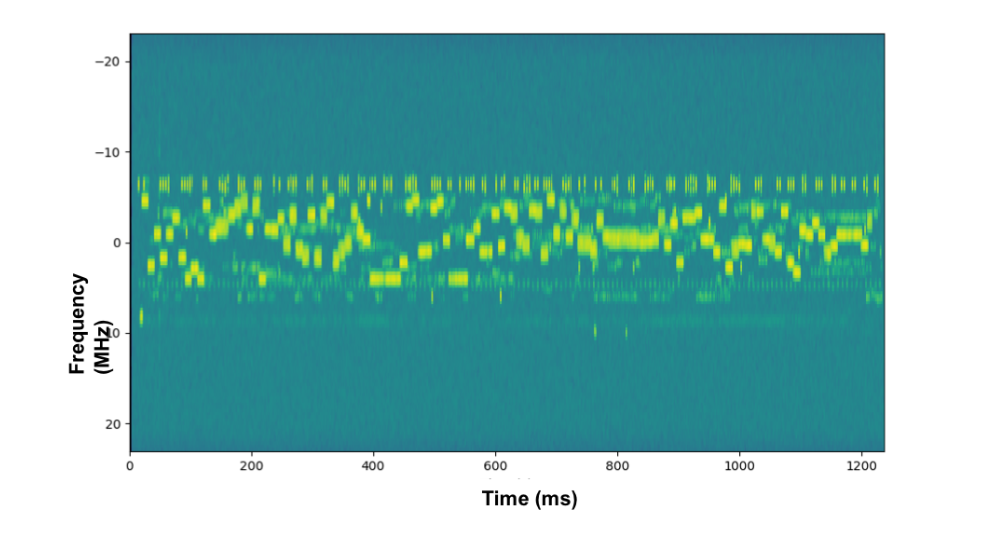
\includegraphics[width = 1.0\textwidth]{Alleys_of_Austin_Channel_Access.PNG}}
    \caption{The spectrum occupied by our network during an Alleys of Austin scenario emulation}
    \label{fig:B.5}
\end{figure}

Post-bandwidth assignment, the channel allocation sub-problem is taken up by the Gateway SRN: it should determine the center frequencies that minimize interference from (and in turn interference to) the other competitors' SRNs in the emulation scenario, while achieving the mandated minimum required throughput and maximum allowable latency QoS constraints imposed on each traffic flow (additional QoS constraints can be imposed on file transfer flows\texttt{-{}-}typically, the time window within which the file transfer needs to be completed from the source SRN to the destination SRN within our network). In order to obtain a complete picture about the spectrum occupancy at a specific SRN in our network (i.e., at a particular location), we exploit two kinds of data: CIL messages from the other competitor networks in the emulation scenario\texttt{-{}-}specifically, the SpectrumUsage messages and the LocationUpdate messages; and the PSD measurements made at the SRN. The Gateway SRN's channel allocation heuristic employs the data gleaned from the SpectrumUsage and LocationUpdate CIL messages broadcasted over the collaboration network by the other competitors in the emulation scenario, and the collated location-specific PSD measurements in the following fashion: first, the channel gain between a pair of SRNs in our network is estimated based on their location information (which is typically obtained from the C2API, if not, it is obtained from the periodic GPS NotificationEvents published by individual SRNs and sent to the Gateway SRN over the high data rate DFT-s-OFDM control link (interleaved with data)) and an empirical path loss exponent; second, based on this estimated channel gain\texttt{-{}-}and a weighted combination of collated PSD measurements and competitor CIL messages\texttt{-{}-}the Gateway SRN determines the amount of interference experienced by our SRNs in each of these channels, and performs a heuristic search to determine the center frequencies that minimize the total interference caused at our SRNs. Fig.\ref{fig:B.5} illustrates the spectrum occupancy of SRNs in our network (as seen by one SRN\texttt{-{}-}collated using PSD measurements and internal occupancy notifications from the Gateway SRN).
\subsection{Multi-hop Routing Heuristic (NET)}\label{B.I.VII}
When the ``short" control messages over the FSK control channel cannot be received by SRN $i$ from SRN $j$ for a pre-determined amount of time (typically, $10$ seconds), the link $l_{ji}$ is reported to be blocked/down by SRN $i$ (similar behavior by all the other SRNs in our network). This routinely occurs in any given DARPA SC2 emulation scenario due to the presence of emulated physical obstacles (hills, buildings, etc.), or the presence of jammers in the network, or the emulation of node mobility characteristics, or high noise and interference in the spectrum as a whole resulting in failed decoding of the short control message packets sent over the FSK control channel (which uses the band-edges of the spectrum). On the other hand, a successful/working link is reported by SRN $i$ with respect to link $l_{ji}$, if short control message packets from SRN $j$ can be successfully decoded. Hence, a binary vector can be constructed at each individual SRN indicating the status of its incoming links\texttt{-{}-}which is then shared with all the other SRNs in the network over the FSK control channel, in order to build a routing table at each SRN, which is periodically updated throughout the emulation.

During data transmission, assuming a correct and current routing table exists at each SRN (which is true because of the periodic updates sent from all the other SRNs over the robust FSK control link), in the Network layer (NET) of each SRN, Dijkstra's algorithm is applied to this routing table, to find the route to the destination SRN using the smallest number of hops.
\section{The Colosseum Command and Control radio API (C2API)}\label{B.II}
The Colosseum Command and Control API (C2API), also referred to as the Radio C2API, is an interface of four shell scripts\texttt{-{}-}namely, start.sh, stop.sh, status.sh, and statistics.sh; which should be supported by every SRN in the deployment, and the combinations of which are used by the scenario emulator, i.e., the Colosseum, in any given deployment, to orchestrate the following activities \cite{DARPA:SC2c2api}:
\begin{itemize}
    \item Notify all the SRNs in the deployment of changes to the radio environment, i.e., changes to the available scenario bandwidth, Passive Incumbent center frequency and threshold changes (discussed in Section \ref{B.I.I}), and scenario stage resets;
    \item Notify all the SRNs in the deployment of their respective newly assigned traffic flows and the QoS constraints (termed ``Individual Mandates (IMs)") for each of them\texttt{-{}-}in addition to performance mandates for a competitor network as a whole (termed ``Network Mandated Outcomes");
    \item Provide static Colosseum configuration information such as the channel emulator's operating frequency, in addition to collaboration network parameters; and
    \item Administration and Management of individual SRNs in individual competitor networks in the deployment, throughout the scenario execution process.
\end{itemize}
\section{The CIRN Interface Language (CIL)}\label{B.III}
As discussed earlier, the DARPA SC2 Grand Challenge involves a collaboration channel (outside the RF environment) that facilitates the cooperative exchange of crucial operational and performance messages among competing CIRNs\texttt{-{}-}in order to not only ensure optimal performance by individual competitor networks, but also by the ensemble, as a whole. By design, every competitor network should have a designated gateway node that communicates with other competitors in the deployment, over the collaboration channel. The gateway SRN corresponding to every competitor network in the deployment will connect to a collaboration server over a wired IP link (ip\_addr:access\_interface), with this collaboration server acting as a publisher-subscriber\texttt{-{}-}tracking competitor SRNs in the deployment, and re-directing peer-to-peer collaboration traffic from the sender gateway to the destination gateway \cite{DARPA:SC2collaboration}.

The collaboration API involves two types of messages \cite{DARPA:SC2collaborationprotocol}:
\begin{itemize}
    \item Client-Server: a set of procedures and semantics to be followed by competitor networks in the deployment, while interacting with the collaboration server in order to ``discover" the addresses of other competitors in the scenario emulation; and
    \item Peer-to-Peer: a set of procedures and semantics that forms the crux of the CIRN Interface Language (CIL) specifications, and is used to describe the collaborative information exchange between two competitor networks in the deployment.
\end{itemize}
The format/structure/semantics of these messages are described in the now standardised CIL protocol specifications. We list a few important collaboration client-server and peer-to-peer messages below:
\begin{itemize}
    \item TalkToServerMessage: All client-server messages, i.e., the messages from a gateway SRN to the collaboration server, should be formatted according to this top-level wrapper\texttt{-{}-}derived instances include Register (a gateway SRN wishes to register its network with the collaboration server), KeepAlive (serves as a heartbeat message from the gateway, informing the collaboration server that it is still active), and Leave (a gateway SRN informs the collaboration server that its network wishes to leave the collaboration channel);
    \item TalkToClientMessage: All messages from the collaboration server to the client are instances of this parent structure\texttt{-{}-}encapsulates Inform (response to Register from the client: the collaboration server sends the unique client ID, maximum keep-alive count, and a list of registered competitors in the collaboration network (i.e., their client IDs and IP addresses); and Notify (the collaboration server broadcasts to all registered clients on the collaboration network that either a new competitor has successfully registered with it, or an existing competitor has left the collaboration channel);
    \item CilMessage: A top-level wrapper encapsulating all peer-to-peer messages in the collaboration network\texttt{-{}-}specifically, IncumbentNotify and IncumbentPassiveInfo (Passive Incumbent messages: discussed in Section \ref{B.I}), LocationUpdate (GPS location information for all SRNs in a competitor network), SpectrumUsage (the exact spectrum voxels, i.e., time-frequency resources, being accessed by SRNs in a competitor network, along with their perceived importance to satisfying the network's assigned mandates), and DetailedPerformance (total number of QoS constraints assigned, total number of QoS constraints satisfied, total score achieved, score threshold for ensemble utility optimization, etc.).
\end{itemize}
\section{Capabilities and Performance Evaluations from DARPA SC2 scenario emulations}\label{B.IV}
In this section, we present plots illustrating the operational capabilities and the performance of our SRNs (and our network, as a whole) in a military deployment scenario, i.e., Alleys of Austin, and a disaster relief deployment scenario, i.e., Wildfire.
\subsection{Alleys of Austin}
This emulated military deployment scenario in the Colosseum, involves a $45$-member platoon (with an Unmanned Aerial Vehicle (UAV)) from the Texas Army National Guard practicing urban maneuvers and communications in Austin, Texas. The platoon is divided into $5$ squads, with $9$ members in each squad, and is moving through the streets of Austin in three stages\texttt{-{}-}involved in basic voice communications in Stage $1$, Stage $2$ involves the exchange of voice, imagery, and video, and Stage $3$ involves a significant increase in the amount of traffic (voice, imagery, and video) exchanged among the squad members. Each competitor CIRN represents a squad\texttt{-{}-}thereby resulting in a $5$ team, $50$ node ($5{\cdot}9{=}45$ SRNs${+}5{\cdot}1{=}5$ gateway SRNs, with an emulated UAV), large-scale, small packet, military deployment scenario, employing a single-tap propagation model \cite{DARPA:SC2scenarios}. Each team must achieve $50$\% of the QoS mandates assigned to it, during the scenario emulation\texttt{-{}-}in a given time snapshot, teams get scores only if every competitor network achieves their corresponding desired performance in that time snapshot, thereby each competitor is incentivized to work with the others in the network in achieving the required mandates.
\begin{figure} [htb]
    \centerline{
    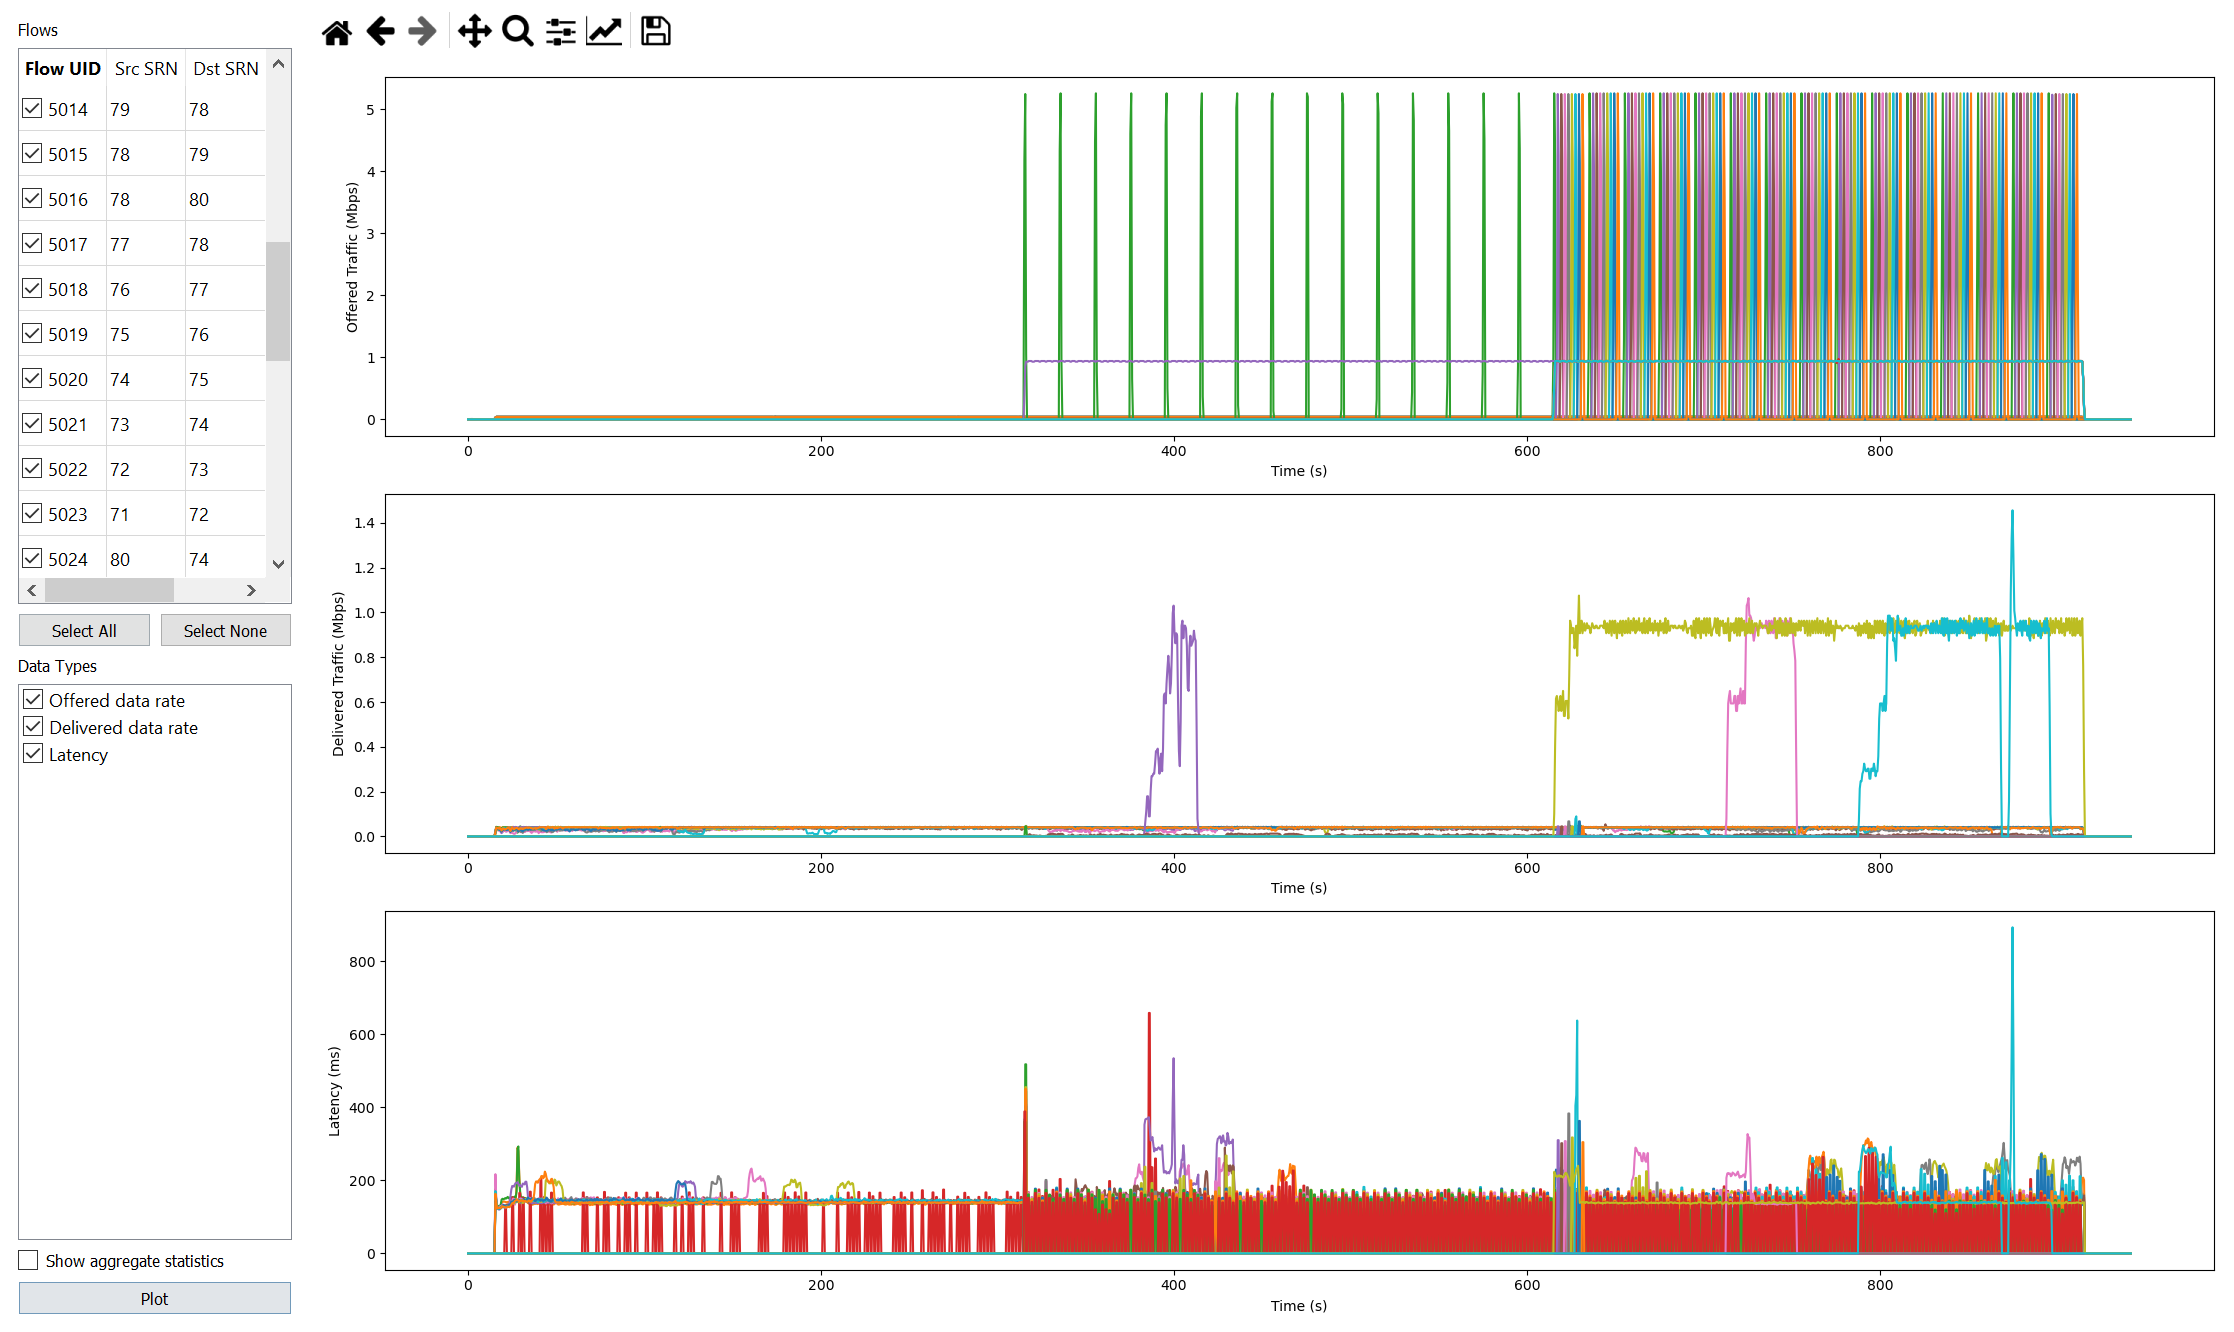
\includegraphics[width = 1.0\textwidth]{Alleys_NET.PNG}}
    \caption{The offered and delivered traffic corresponding to various (selected) flows during the Alleys of Austin scenario emulation}
    \label{fig:B.6}
\end{figure}

Fig. \ref{fig:B.6} illustrates the offered traffic corresponding to the individual selected flows, their corresponding delivered traffic, and the latency experienced by these flows as they are being scheduled/delivered by our network. Note here that our network is able to deliver almost all of these flows with minimal latency. Also, note the stages in the scenario emulation\texttt{-{}-}as described earlier, Stage $1$ constitutes basic voice traffic, i.e., the initial flows have a low offered traffic data rate of $40$kbps; Stage 2 constitutes voice, imagery, and video traffic, i.e., the flows in this Stage have low offered traffic data rate, but imagery and video flows carry higher point values (flow priorities); and finally Stage $3$ involves a significant increase in the amount of offered traffic for the voice, imagery, and video flows. From Fig. \ref{fig:B.6}, we observe that our network is able to deliver most of the flows in Stages $1$ and $2$\texttt{-{}-}however, in Stage $3$, as is usually expected, due to the extremely high offered traffic, our network is not able to satisfy all the assigned flows.
\begin{figure} [htb]
    \centerline{
    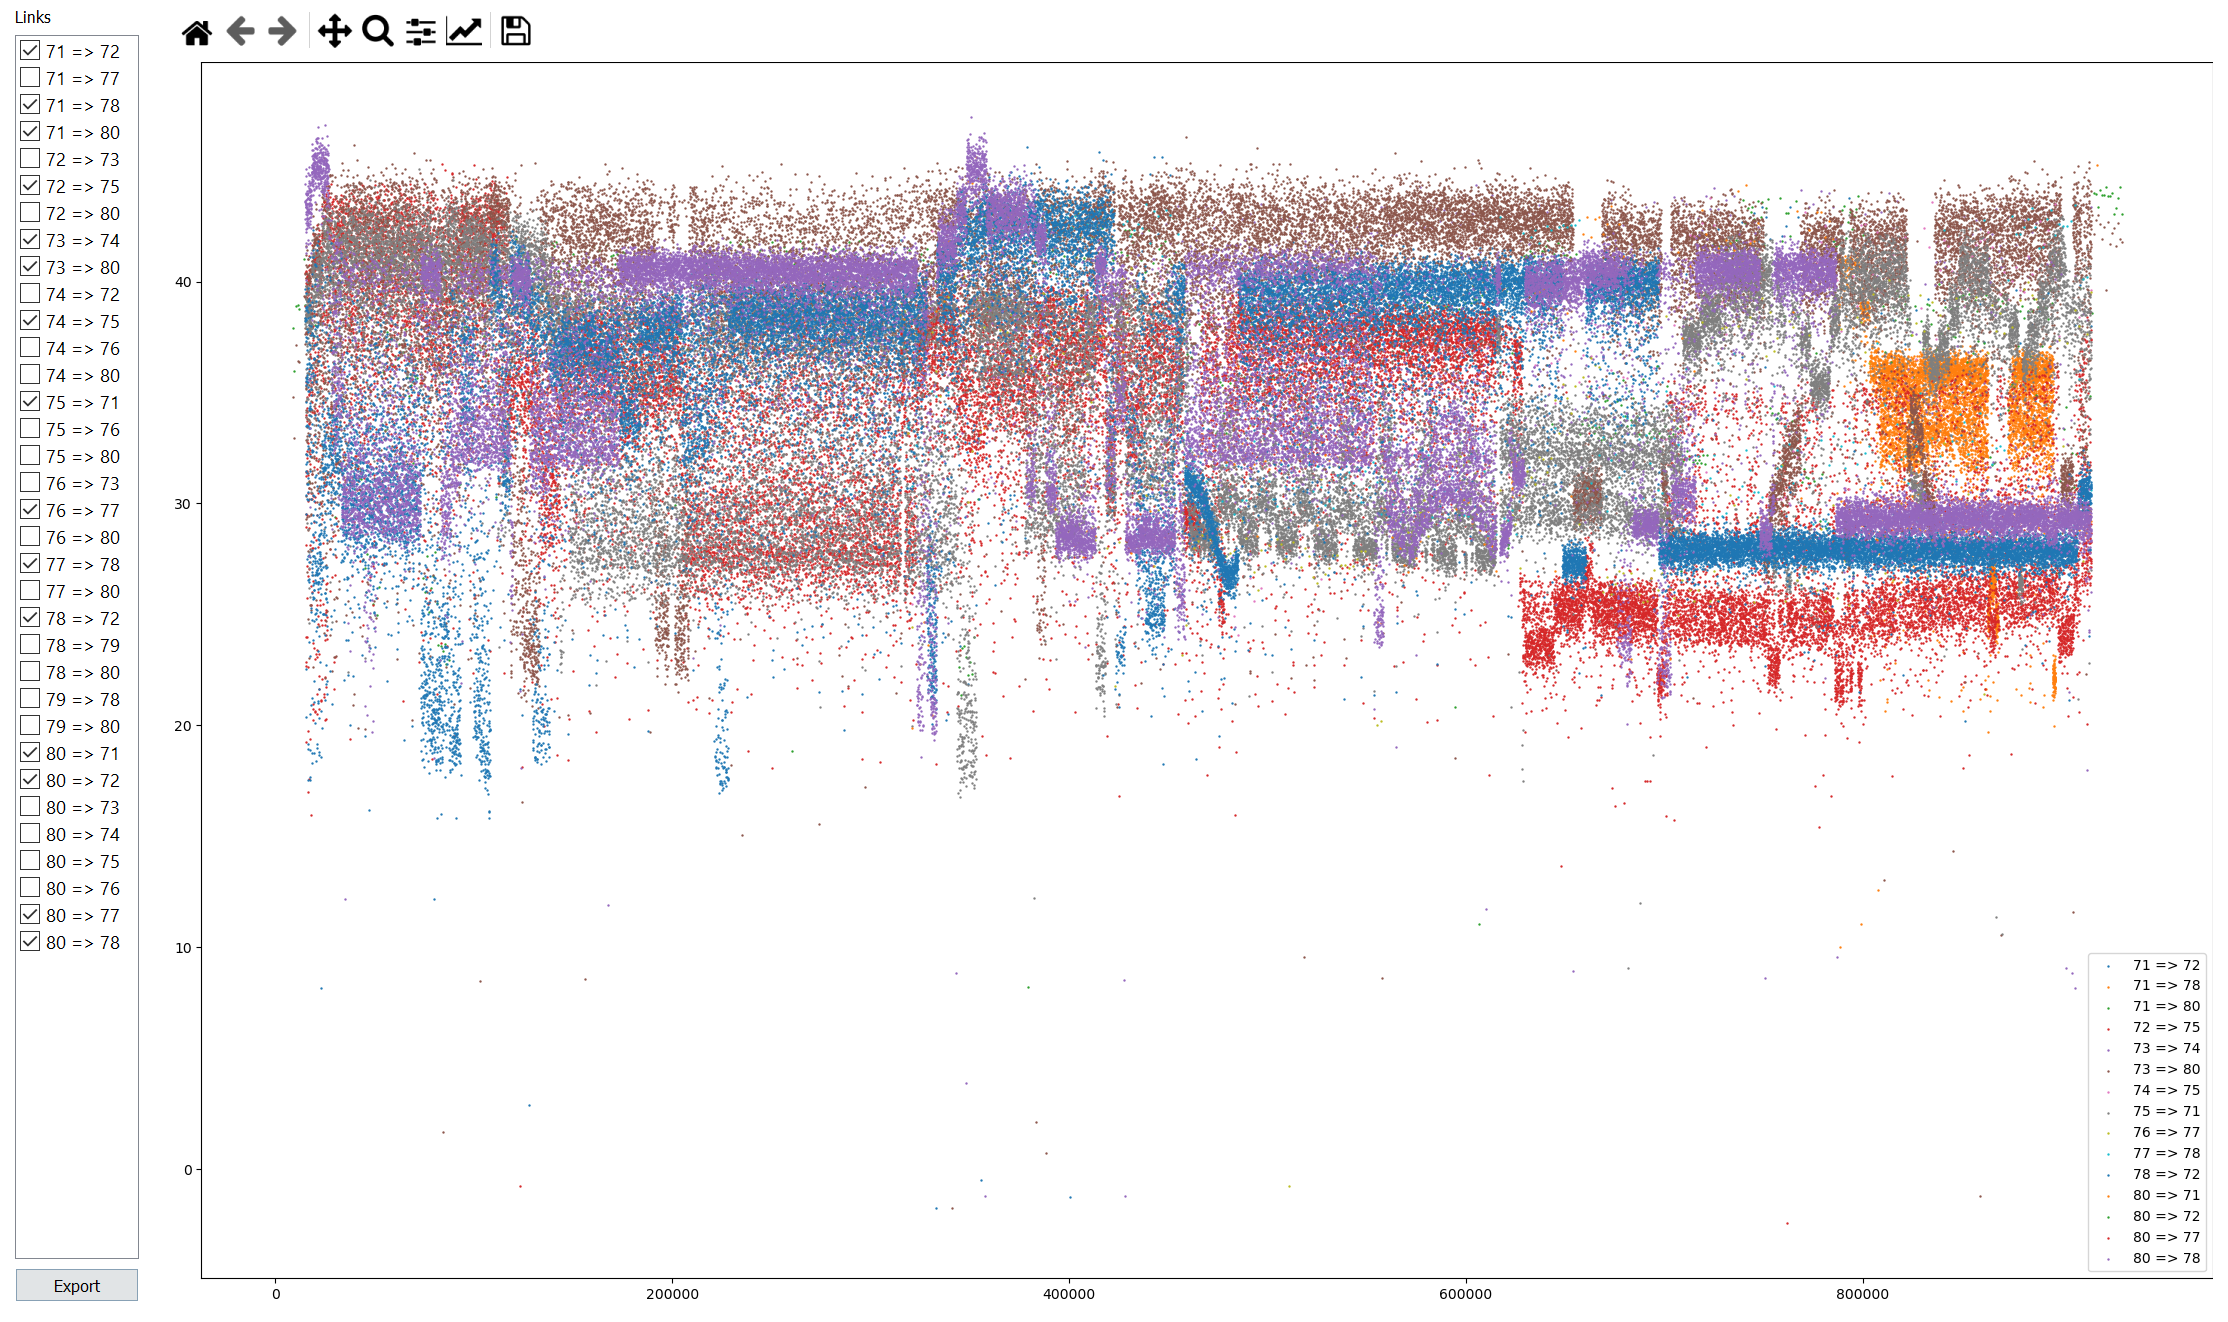
\includegraphics[width = 1.0\textwidth]{Alleys_SNR.PNG}}
    \caption{The estimated SNR on various (selected links) during the Alleys of Austin scenario emulation}
    \label{fig:B.7}
\end{figure}
\begin{figure} [htb]
    \centerline{
    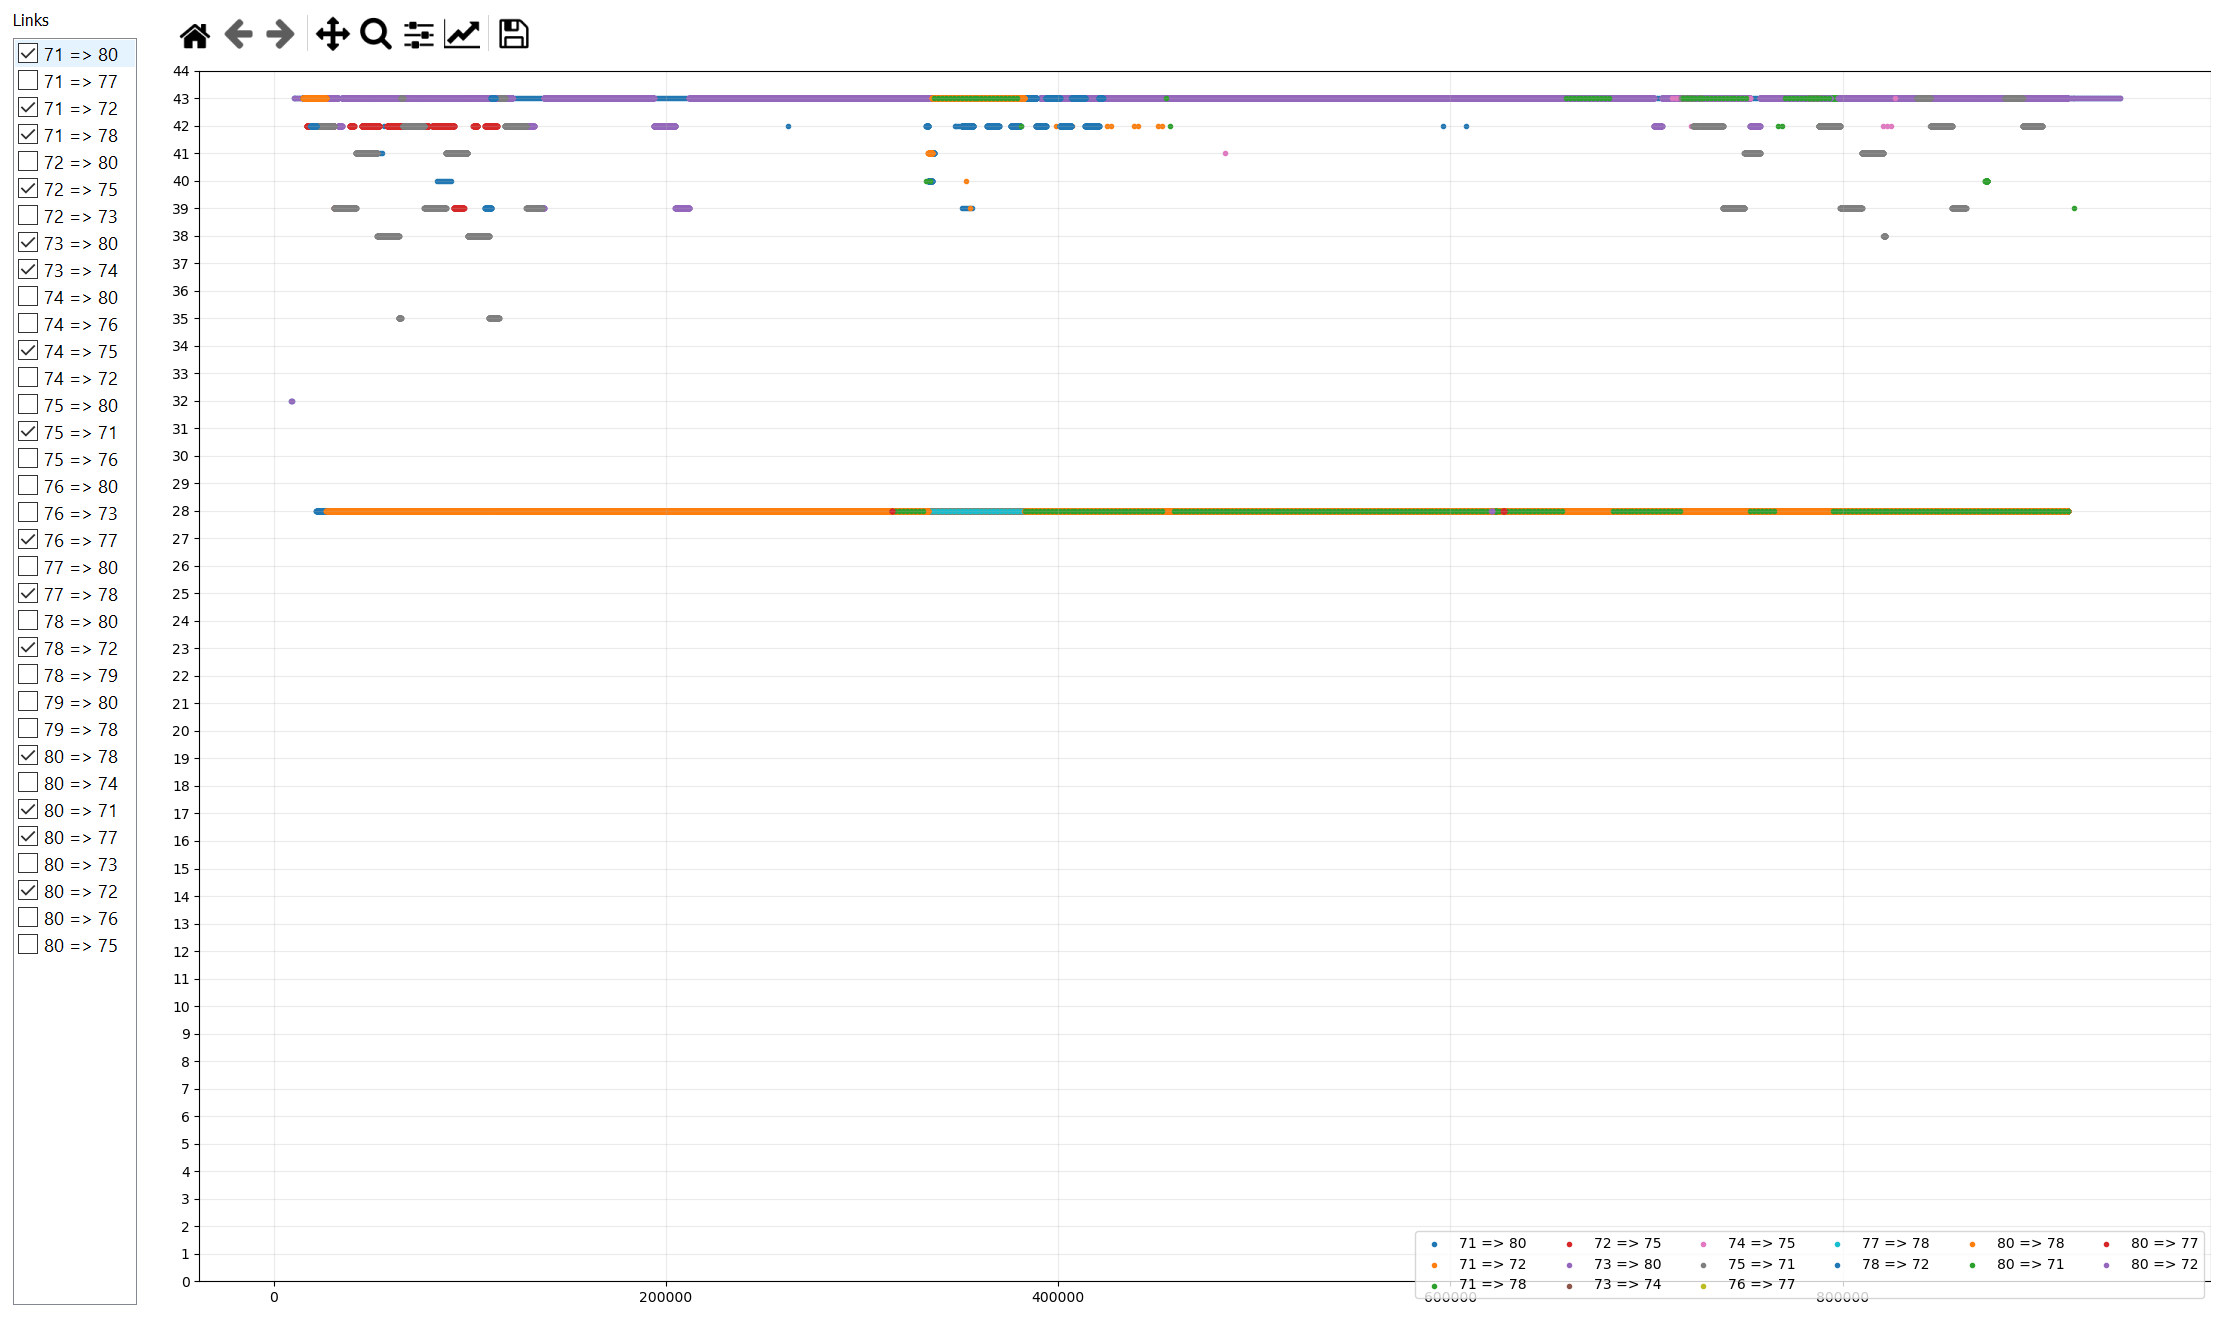
\includegraphics[width = 1.0\textwidth]{Alleys_MCS.PNG}}
    \caption{The MCS adaptation scheme at each (selected) link during the Alleys of Austin scenario emulation}
    \label{fig:B.8}
\end{figure}

Fig. \ref{fig:B.7} depicts the estimated SNR on various selected links (source SRN - destination SRN), during the progression of the Alleys of Austin scenario\texttt{-{}-}these SNR estimates at each link are, as discussed earlier, employed in the MCS adaptation scheme, the prioritized flow scheduler, and the bandwidth allocation algorithm. Consequently, Fig. \ref{fig:B.8} depicts the MCS adaptation scheme at each of these selected links, adapting to the changing estimated SNR with respect to the corresponding channels used by these links\texttt{-{}-}the Y-axis of the MCS adaptation plot in Fig. \ref{fig:B.8} refers to the C${++}$ enumeration value corresponding to the $(\mathcal{M},\mathcal{R})$ pair, i.e., for example, $43$ in the plot refers to QAM$64$ modulation with a code rate of $\frac{5}{6}$, while $28$ refers to QPSK modulation with $\frac{1}{2}$ code rate\texttt{-{}-}in other words, the highest modulation order used in this Alleys of Austin run is $\mathcal{M}{=}64$ (i.e., QAM$64$), while the lowest modulation order used in $\mathcal{M}{=}4$ (i.e., QPSK).
\begin{figure} [htb]
    \centerline{
    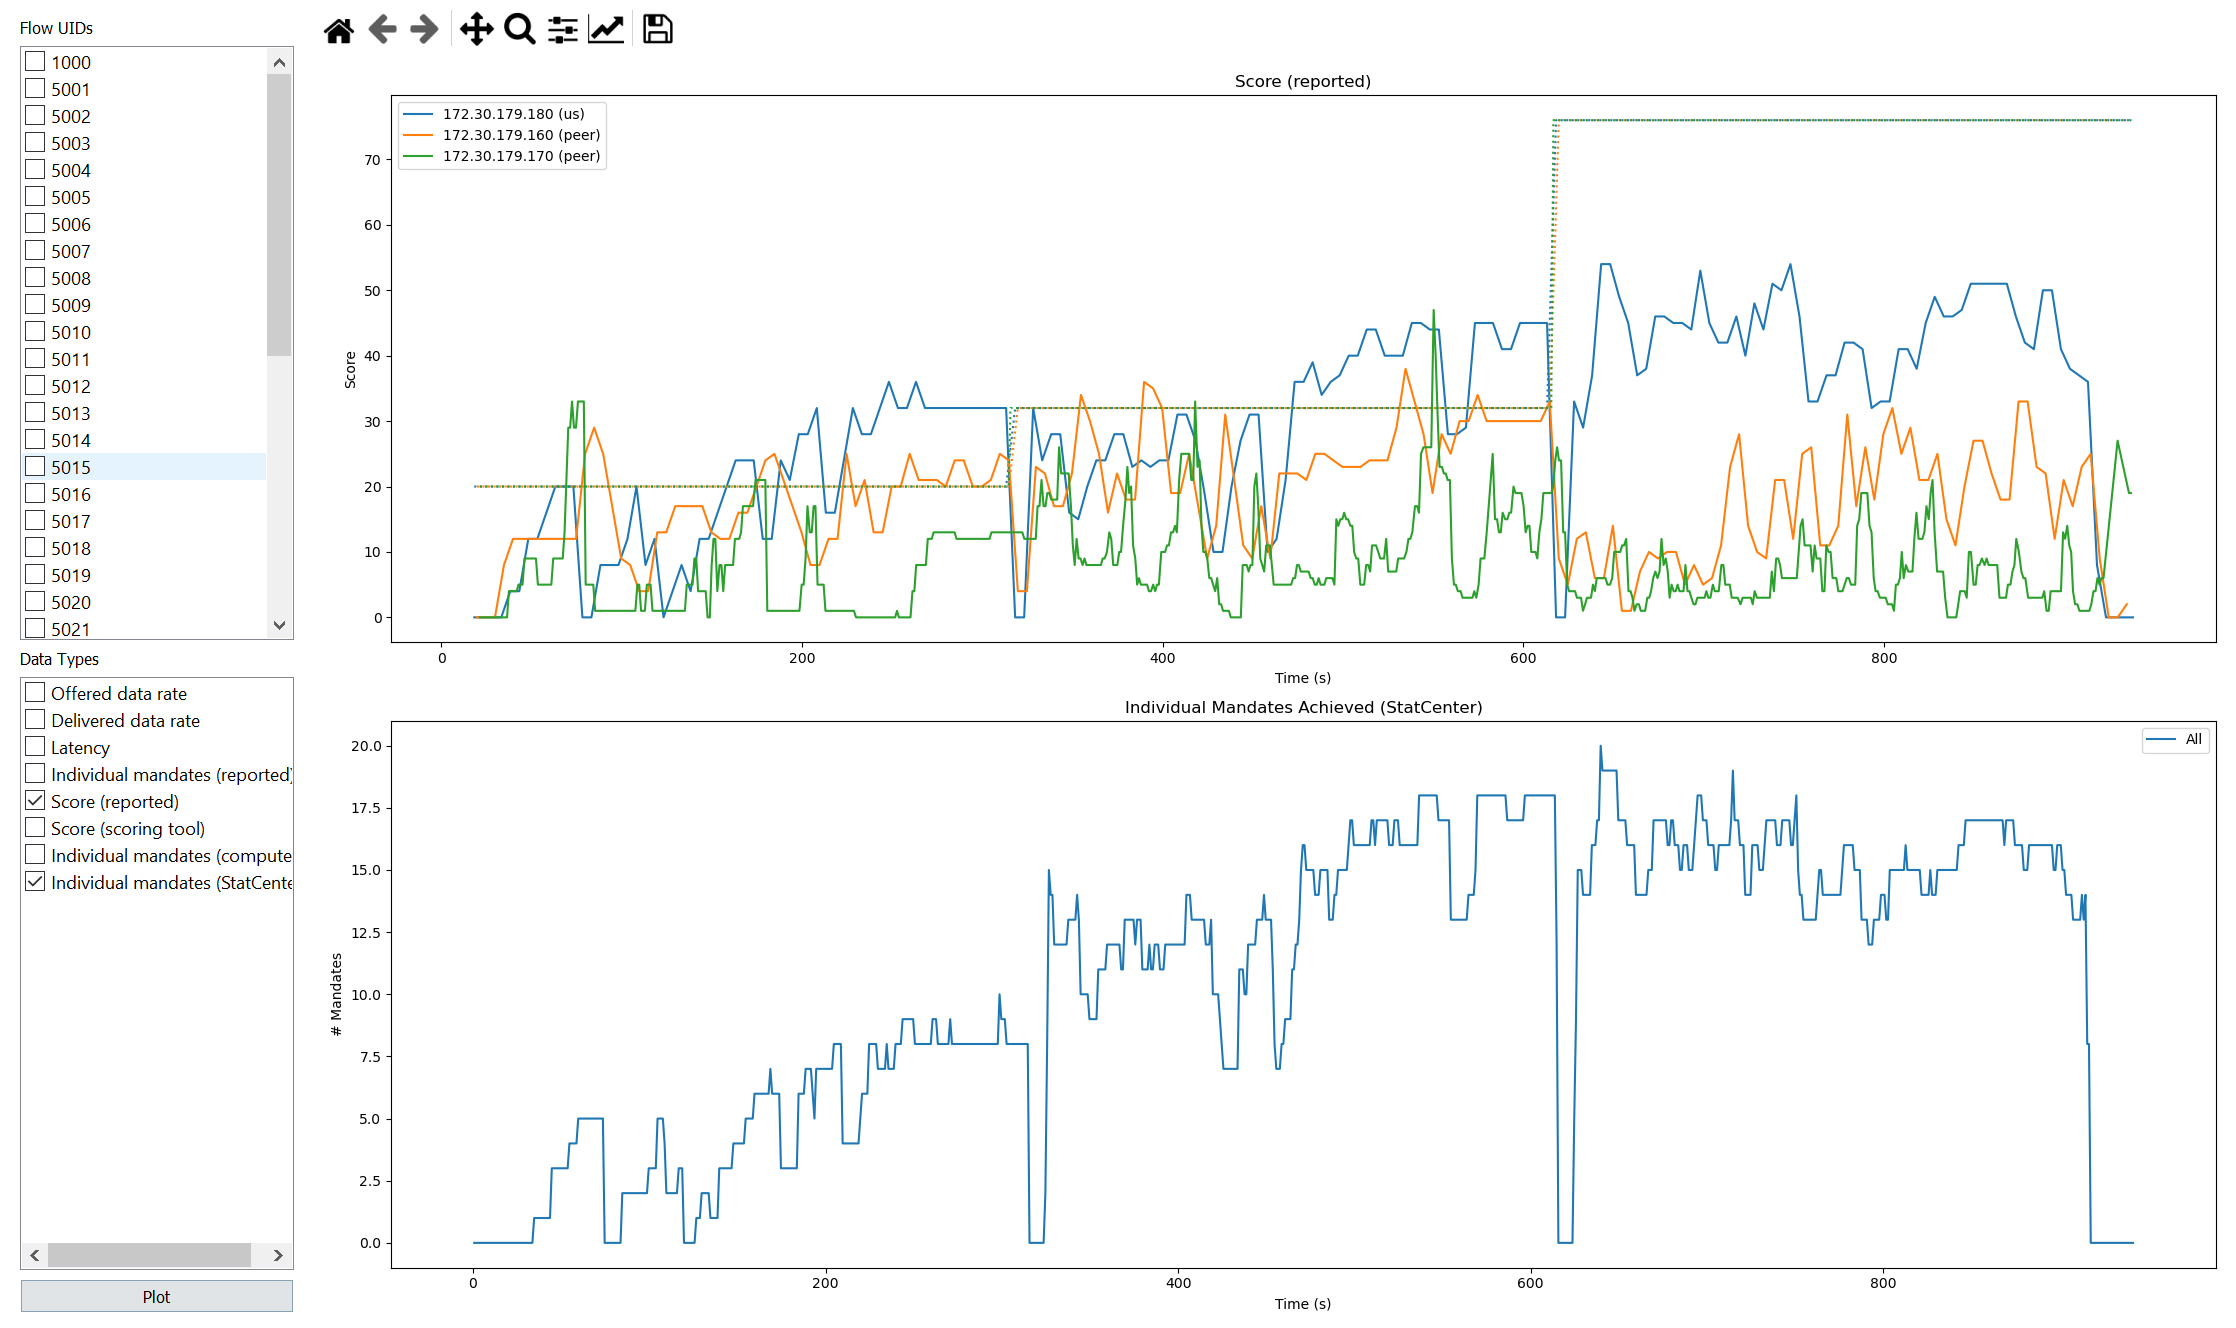
\includegraphics[width = 1.0\textwidth]{Alleys_Scoring.PNG}}
    \caption{The scores attained by our network and other competing networks during the Alleys of Austin scenario emulation, in addition to the number of QoS mandates satisfied by our network in a given time snapshot}
    \label{fig:B.9}
\end{figure}

Fig. \ref{fig:B.9} illustrates the score obtained by our network (indicated by our Gateway SRN's IP address) along with the scores obtained by our peers (indicated by the IP addresses of their corresponding gateway SRNs) in the scenario emulation. The dotted lines in the first sub-plot indicate the score thresholds that need to be achieved by each network, in a Stage. As is evident from the figure, our network satisfies/exceeds the score threshold in Stages $1$ and $2$, but fails in Stage $3$\texttt{-{}-}however, our network does have the best performance among all the teams in the scenario emulation. It is important to note here that even though there were $5$ teams in the emulation of this Alleys of Austin scenario, only the scores of $3$ of them are visualized in this figure\texttt{-{}-}$2$ teams did not report their scores over the collaboration network, and hence their scores were not visualized in this illustration. The second sub-plot illustrates the number of flow-specific QoS mandates that were achieved by our network in a given time snapshot.
\begin{figure} [htb]
    \centerline{
    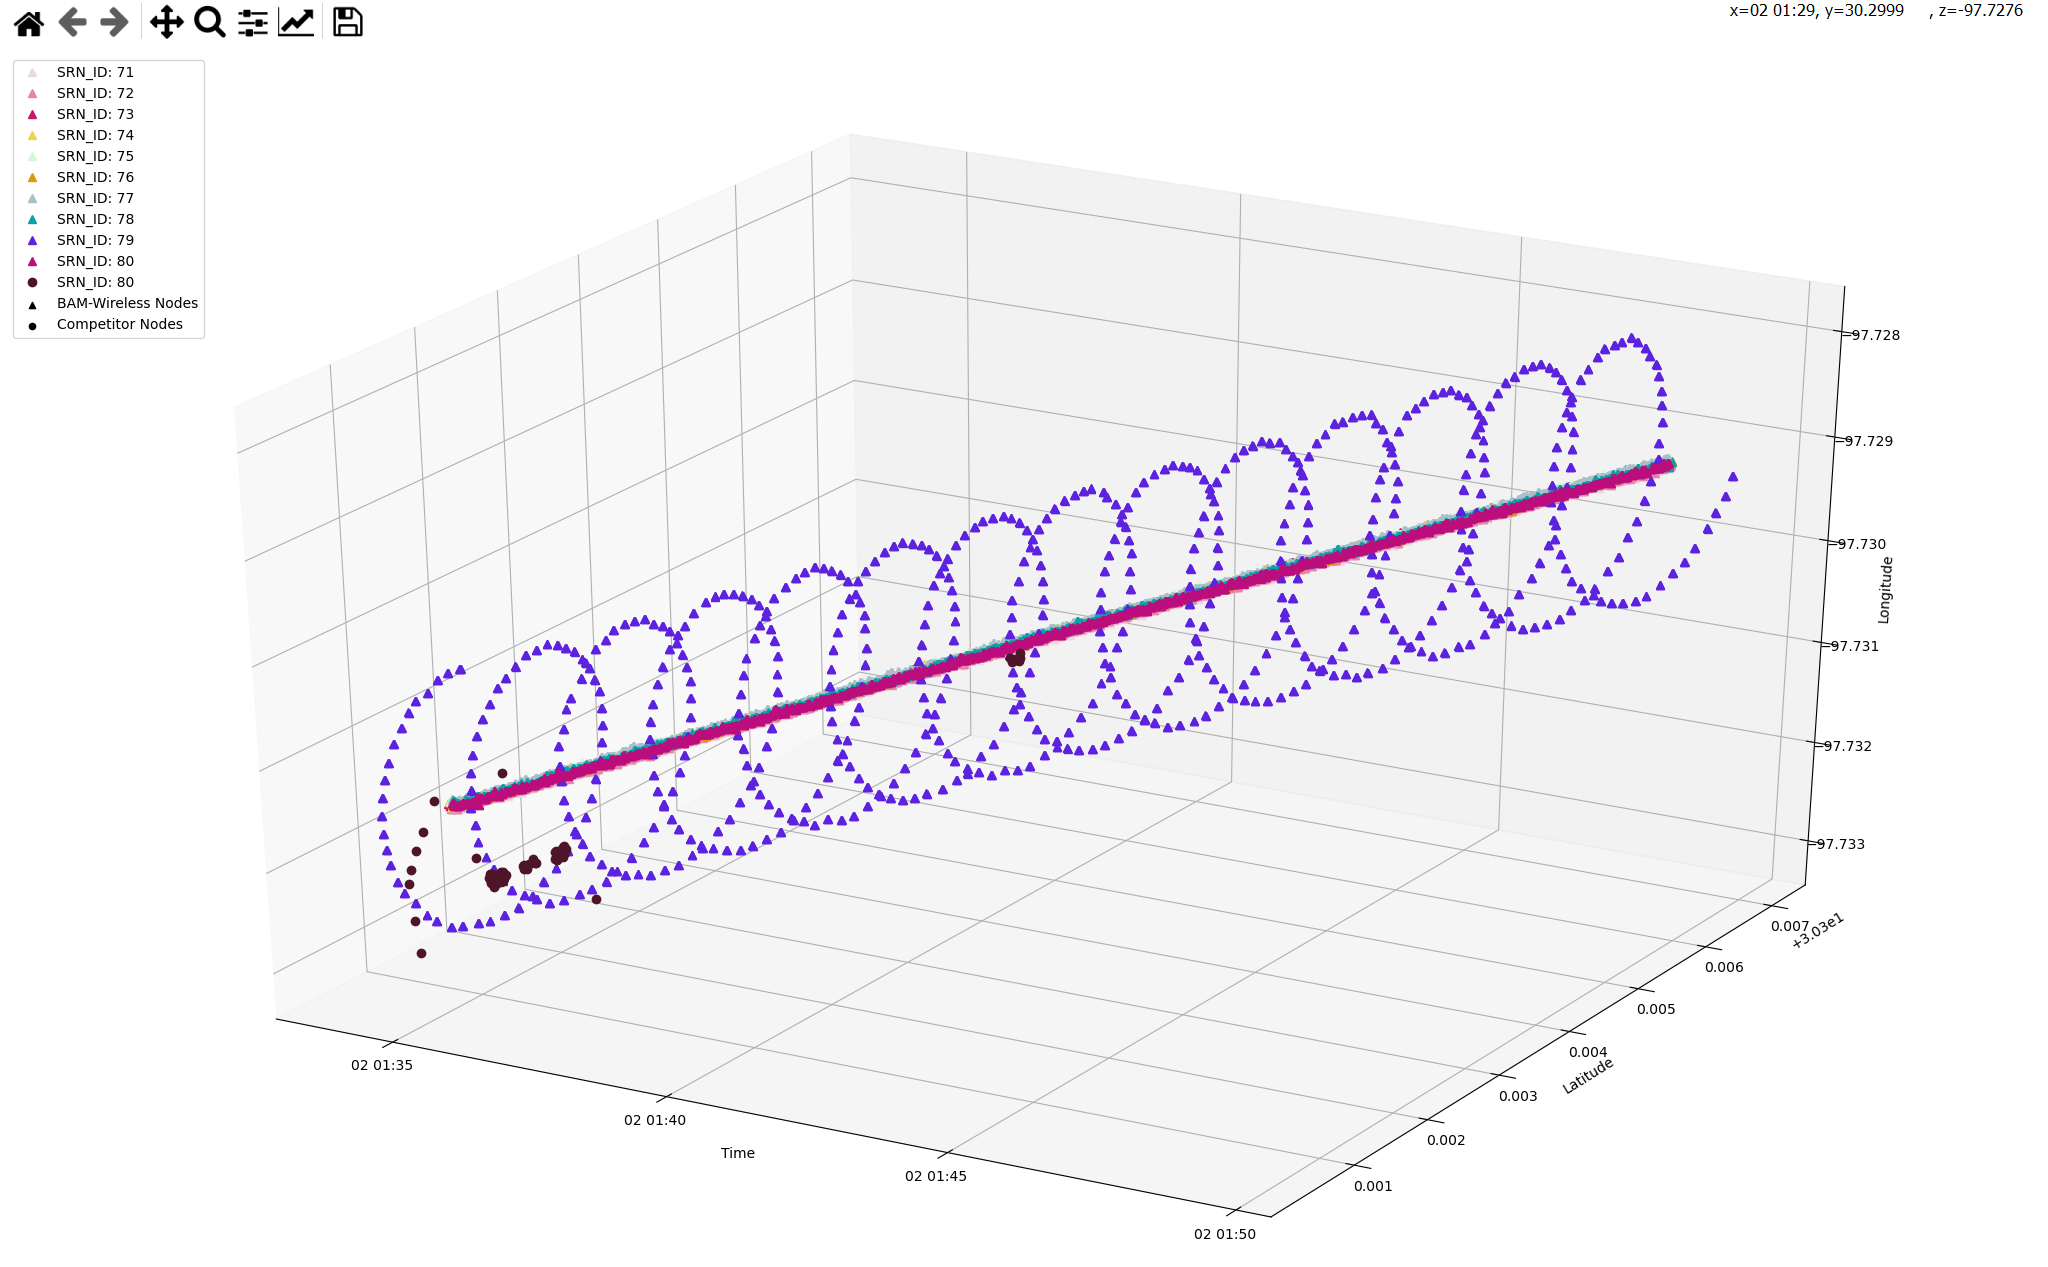
\includegraphics[width = 1.0\textwidth]{Alleys_GPS.PNG}}
    \caption{The reported GPS locations of our SRNs, in addition to those of our competing SRNs, during the Alleys of Austin scenario emulation}
    \label{fig:B.10}
\end{figure}
\begin{figure} [htb]
    \centerline{
    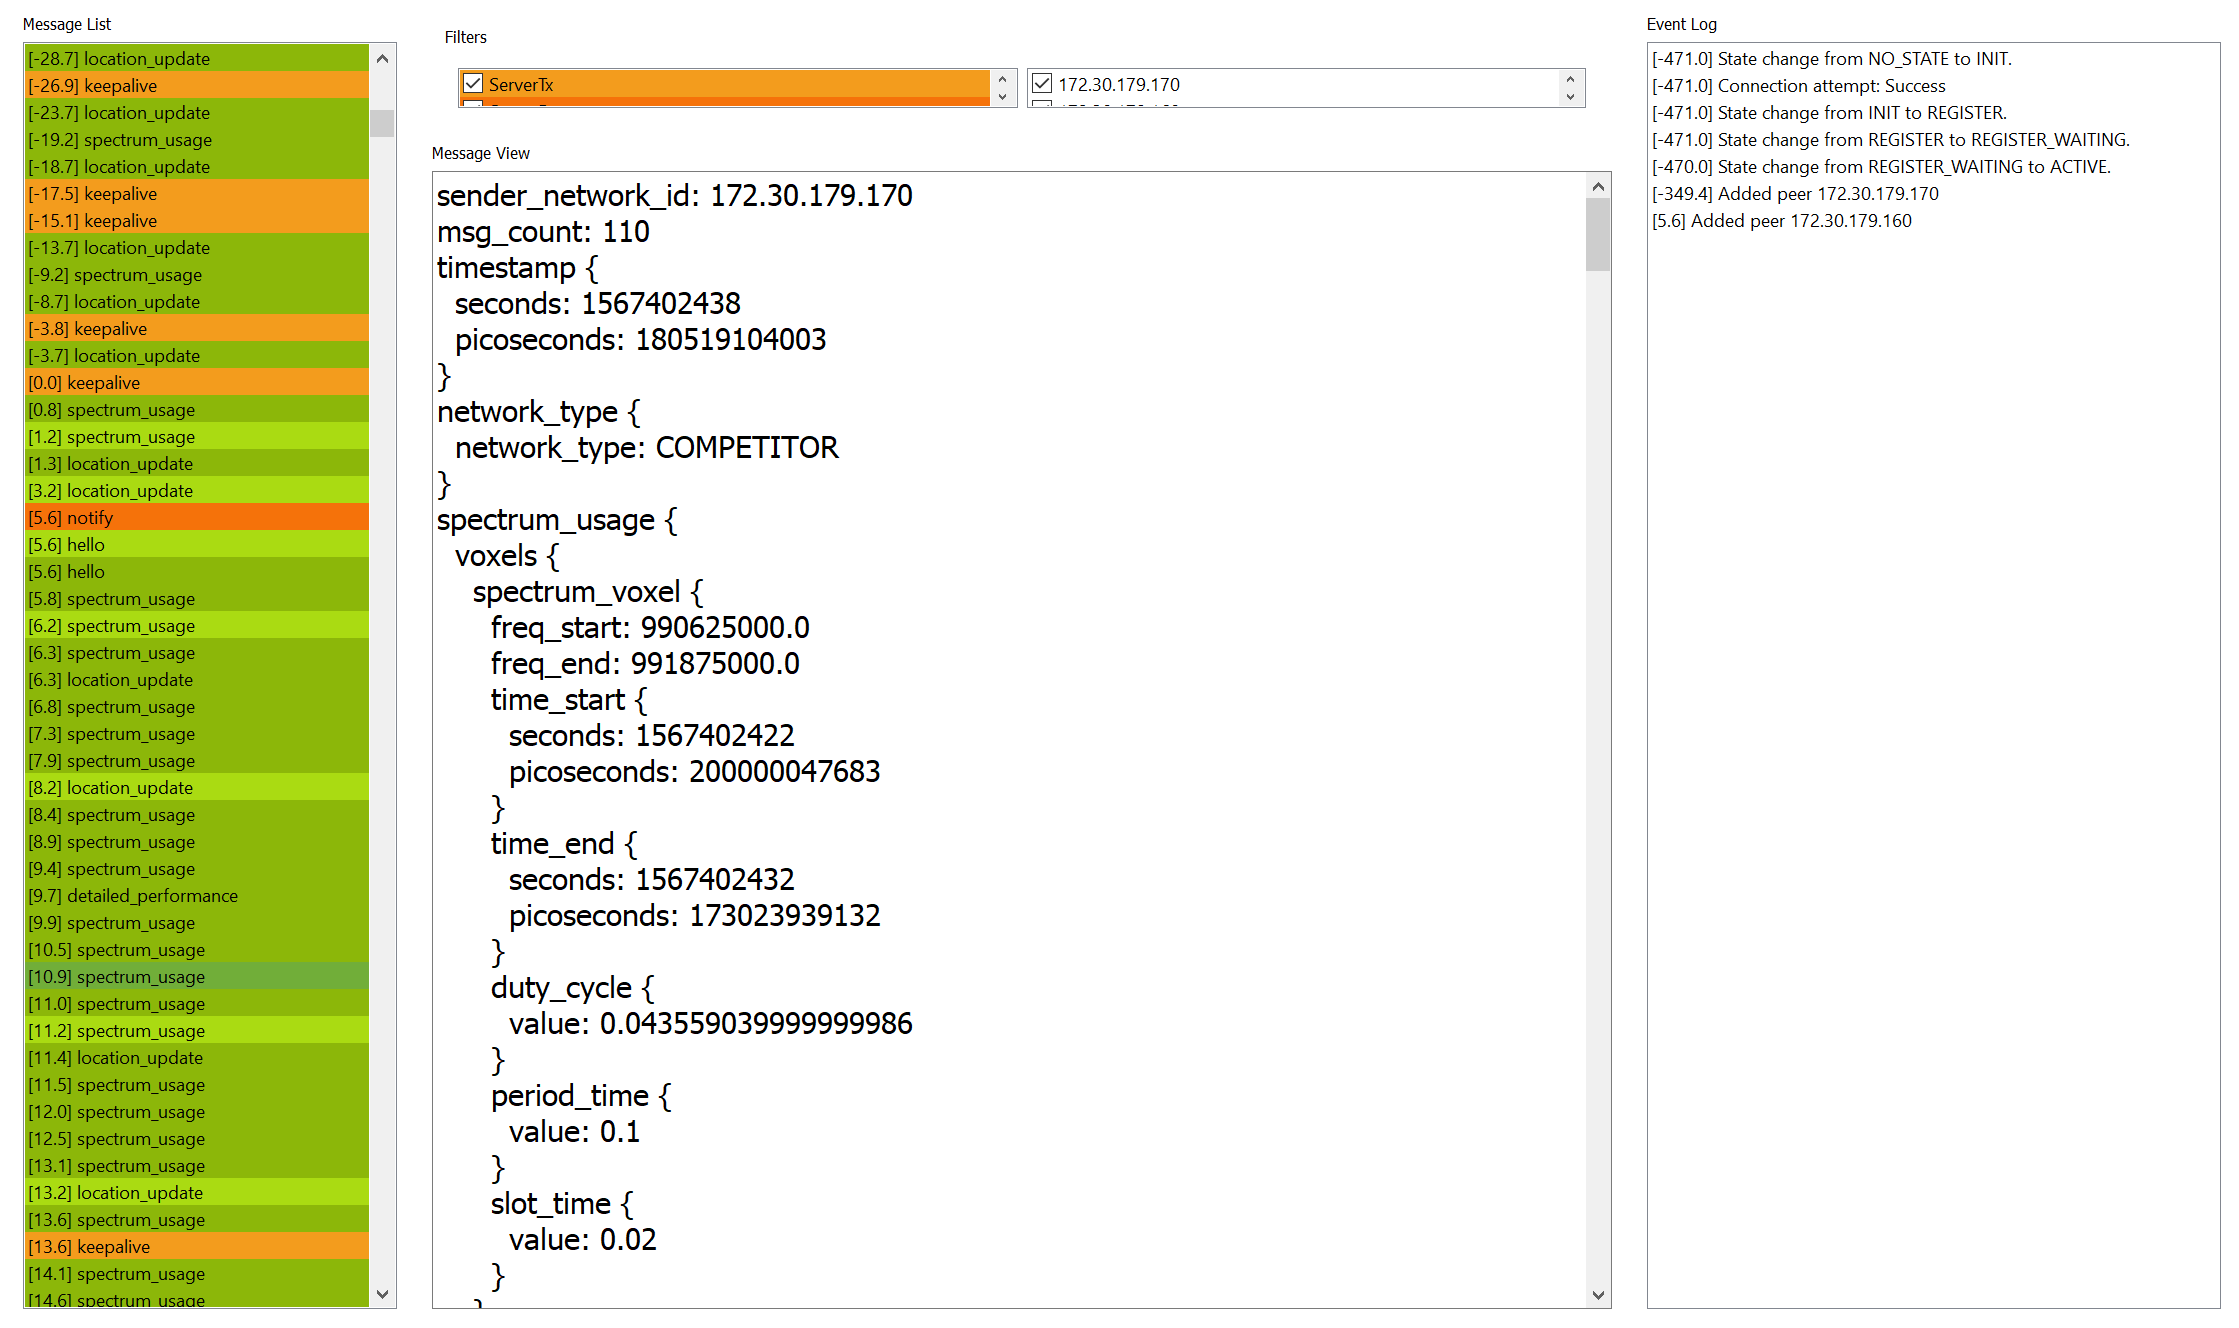
\includegraphics[width = 1.0\textwidth]{Alleys_Collab.PNG}}
    \caption{The description of various CIL message exchanges between our network and the collaboration server, in addition to those between our network and our peers, during the Alleys of Austin scenario emulation}
    \label{fig:B.11}
\end{figure}
\begin{figure} [htb]
    \centerline{
    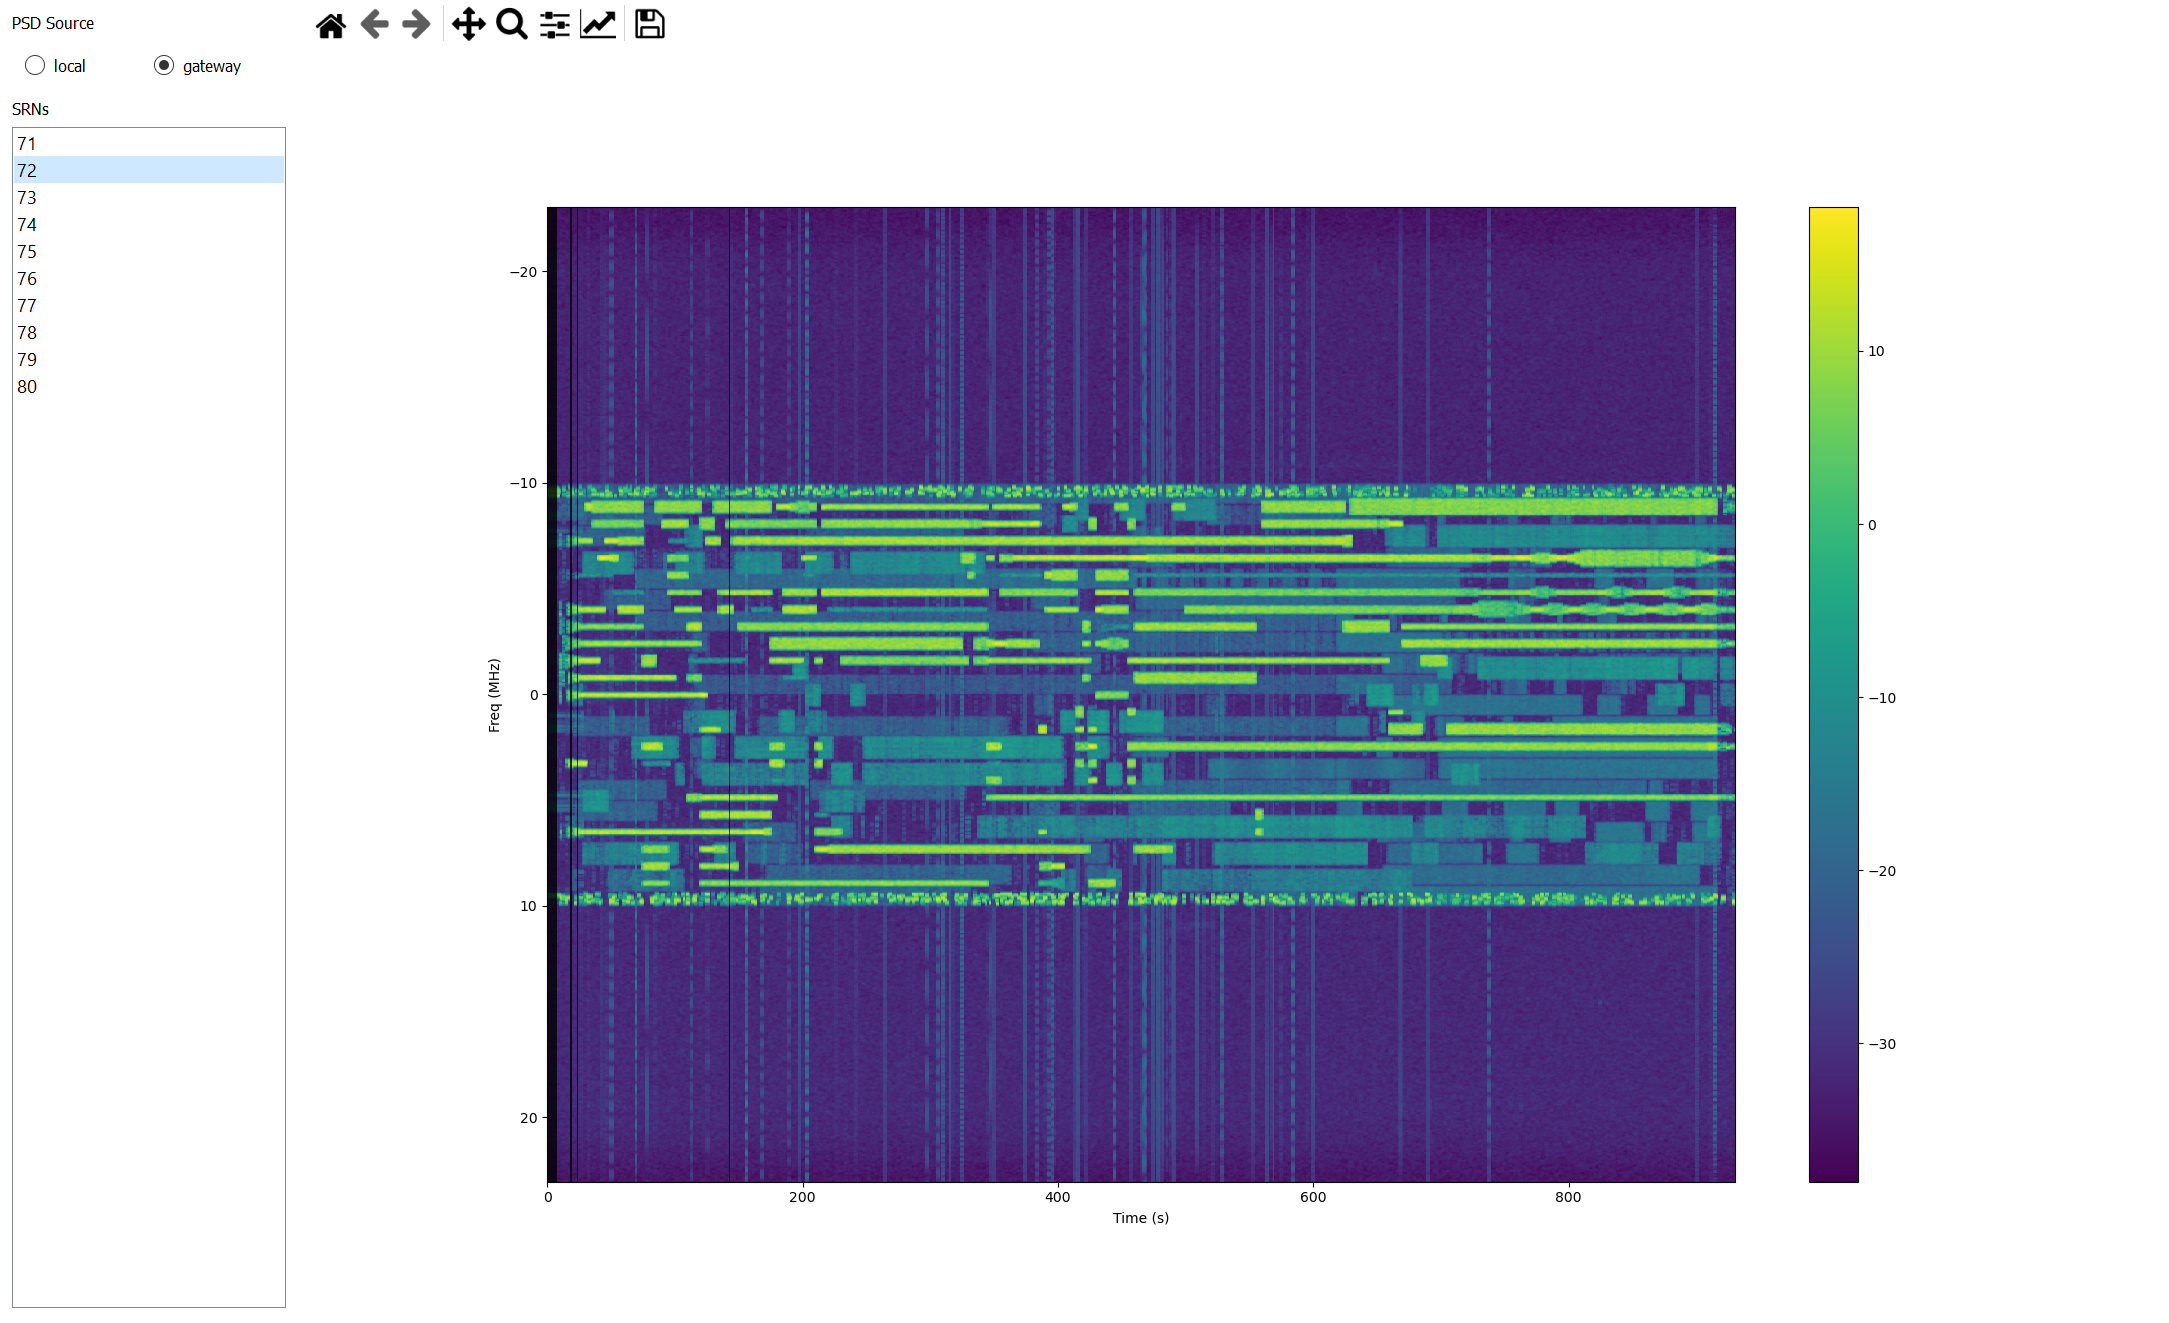
\includegraphics[width = 1.0\textwidth]{Alleys_PSD.PNG}}
    \caption{The PSD measurements received at our Gateway SRN from one particular SRN in our network (selected), in order to obtain location-specific spectrum occupancy information, during the Alleys of Austin scenario emulation}
    \label{fig:B.12}
\end{figure}
\begin{figure} [htb]
    \centerline{
    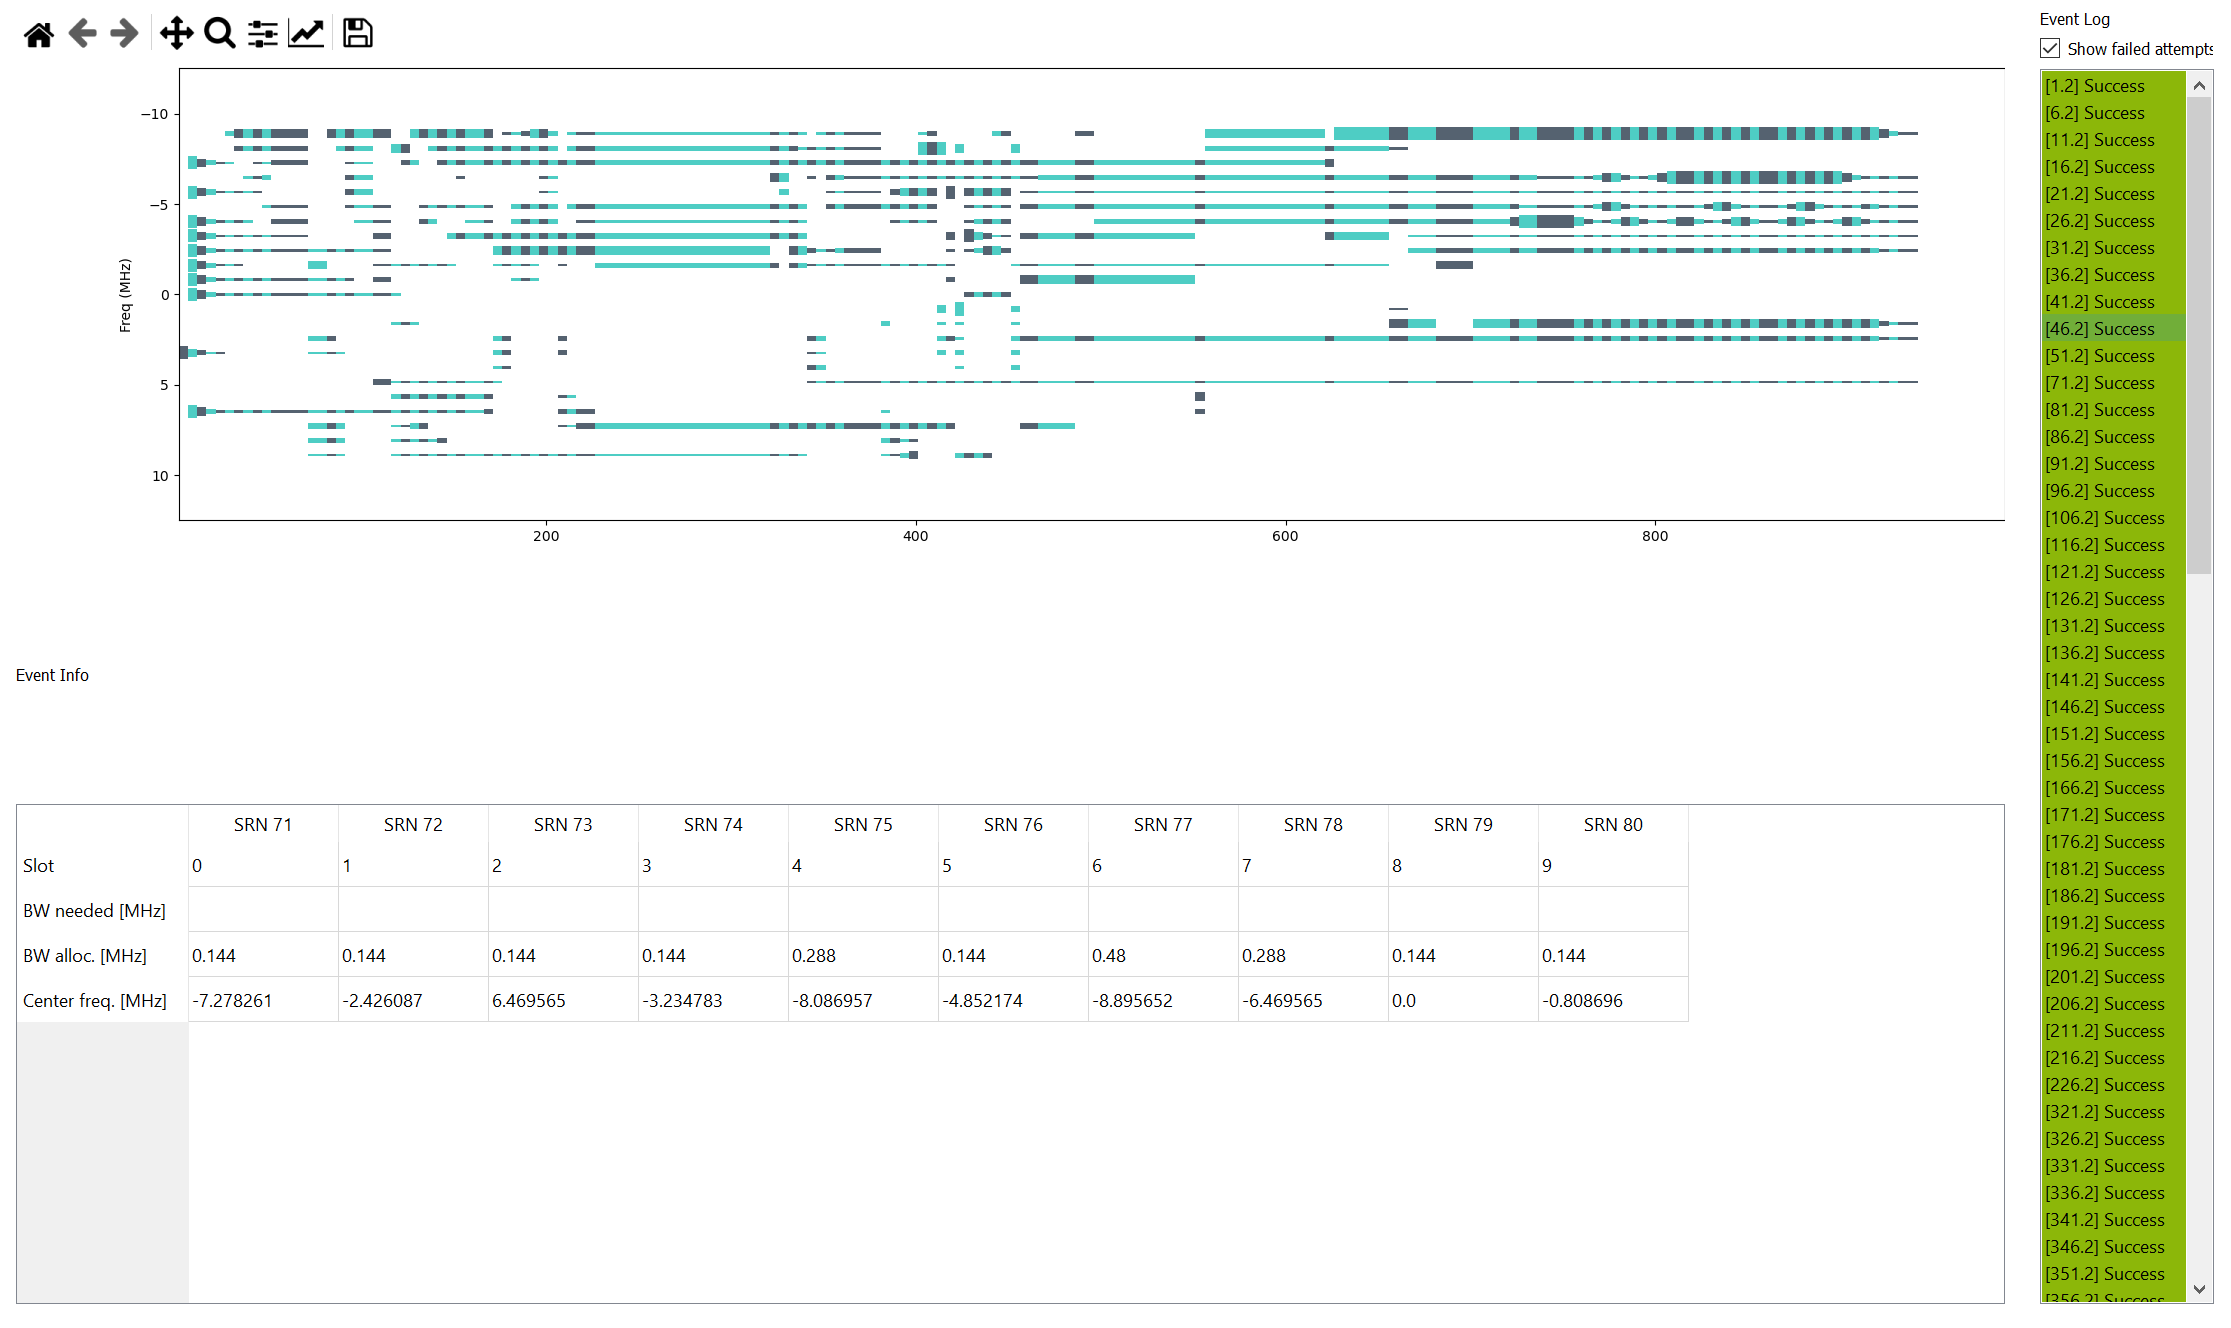
\includegraphics[width = 1.0\textwidth]{Alleys_Channel_Alloc.PNG}}
    \caption{The spectrum occupancy behavior of SRNs in our network (as guided by our Gateway SRN) during the Alleys of Austin scenario emulation}
    \label{fig:B.13}
\end{figure}
The reported GPS locations (latitude, longitude) of the SRNs in our CIRN, and the SRNs in our competitors' CIRNs, over time, are depicted in a $3$-dimensional time plot shown in Fig. \ref{fig:B.10}. The location information of these SRNs\texttt{-{}-}particularly, in relation to physical obstacles (emulated) and competitor SRNs, is employed in the channel allocation algorithm in our Gateway SRN. Fig. \ref{fig:B.11} illustrates the various timestamped CIL messages (both Client-Server messages and Peer-to-Peer messages) received by our Gateway SRN over the collaboration network\texttt{-{}-}these messages are exploited by our Gateway SRN, which along with the collated location-specific PSD measurements: one such PSD measurement in a given time snapshot observed at SRN with ID\texttt{-}$72$ and sent to our Gateway, is depicted in Fig. \ref{fig:B.12}\texttt{-{}-}determines a channel allocation (center frequencies) that minimizes the total interference caused at our SRNs by our competitors. Consequently, from an overall scenario duration perspective, the channel allocations of our network are collated into one ``big-picture" illustration, shown in Fig. \ref{fig:B.13}. It is evident from Fig. \ref{fig:B.13} that in Stage $1$, there are frequent channel re-allocations and bandwidth adjustments, as evidenced by the breaks in the beginning of the plot\texttt{-{}-}this is due to the fact that all the networks, including ours, are trying to find an ``equilibrium" allocation that not only helps them achieve their mandates, but also ensures that the ensemble, as whole, achieves its score threshold; Stage $2$ has a stable channel and bandwidth allocation, as evidenced by the lower number of breaks in the middle of the plot, due to ``equilibrium" being achieved by our network and still a lower amount of traffic, similar in scale to Stage $1$; and finally, in Stage $3$, the significant increase in the offered traffic of all three flows (voice, imagery, and video) places an enormous strain on the limited available RF spectrum allotted for this scenario emulation, and since all teams are vying for the same spectrum resources all the time, due to the increased offered traffic, we see significant breaks towards the end of the plot, indicating frequent bandwidth adjustments and channel re-allocations\texttt{-{}-}this causes poor performance in Stage $3$, as seen in Fig. \ref{fig:B.6} and Fig. \ref{fig:B.9}, but our network still outperforms our competitors in this Stage.
\subsection{Wildfire}
This scenario emulates a disaster-relief deployment\texttt{-{}-}$5$ National Guard units have been deployed to the Lake Sutherland area in Washington in order to fight a wildfire that is raging there. Each of these $5$ National Guard teams are equipped with an Aerostat to assist in communications, and $4$ water-bombers (unmanned water tankers) to put out the blaze. This scenario emulation involves $6$ stages: the water-bombers get into position in Stage $1$; and in Stages $2-6$, $5$ water-bombers from $2$ teams are sent to drop their load onto the blaze, during which these $5$ water-bombers stream high-definition video back (Video\_Bombing\_Run flows\texttt{-}15 points per flow) to the Aerostat (i.e., the unit command and control center), while the remaining loitering $15$ water-bombers send out basic pings to the Aerostat\texttt{-{}-}after dropping their load onto the fire, these $5$ water-bombers come back to their initial position to reload, the next $5$ go out to drop their load, and the process continues until the end of this scenario emulation. Each competitor CIRN represents a National Guard unit\texttt{-{}-}thereby resulting in a $5$ team, $50$ node, large-scale, small packet, disaster-relief deployment scenario, employing a single-tap propagation model \cite{DARPA:SC2scenarios}. Each team must achieve $50$\% of the QoS mandates assigned to it, during the scenario emulation\texttt{-{}-}in a given time snapshot, teams get scores only if every competitor network achieves their corresponding desired performance in that time snapshot, thereby each competitor is incentivized to work with the others in the network in achieving the required mandates. Note here that the main challenge in this scenario emulation is to collaborate with our competitors in this deployment in order to ensure that the ``active" SRNs, i.e., the water-bombers that are sent out to drop their load get most of the spectrum because of the high-definition video flows communicated by these ``active" water-bombers to the Aerostat, are emulated/modeled to need ${\sim}20$\% of the total allocated scenario bandwidth\texttt{-{}-}therefore, teams must work together to facilitate efficient allocation of resources to these ``active" SRNs in any given time snapshot \cite{DARPA:SC2scenarios}.
\begin{figure} [htb]
    \centerline{
    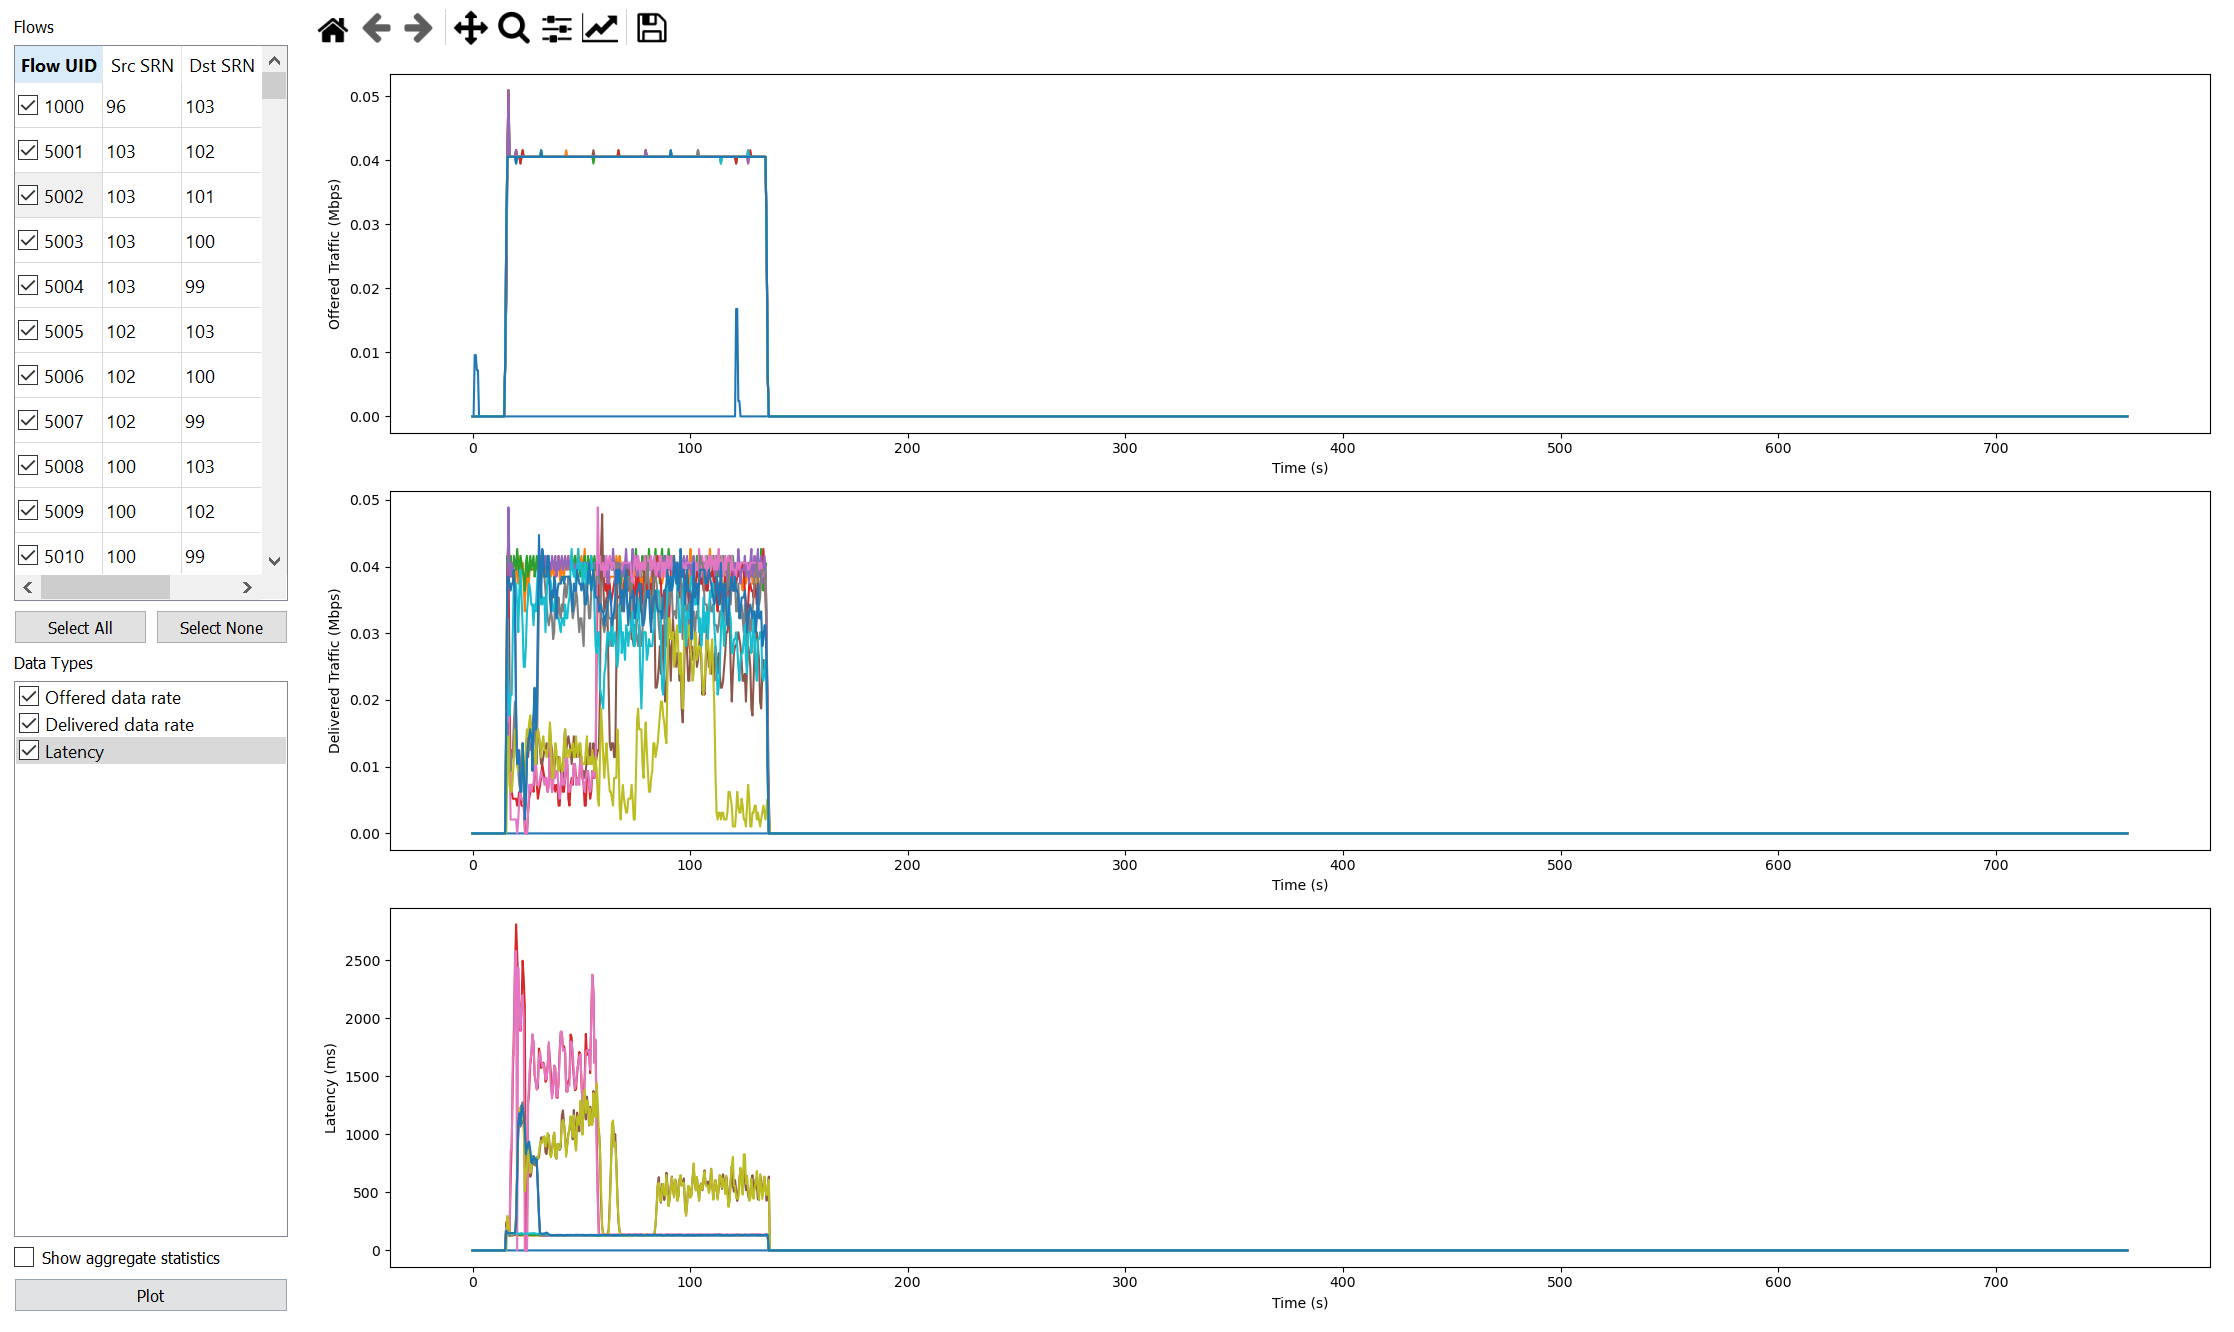
\includegraphics[width = 1.0\textwidth]{Wildfire_NET.PNG}}
    \caption{The offered and delivered traffic corresponding to various (selected) links during the Wildfire scenario emulation (Stage $1$)}
    \label{fig:B.14}
\end{figure}
\begin{figure} [htb]
    \centerline{
    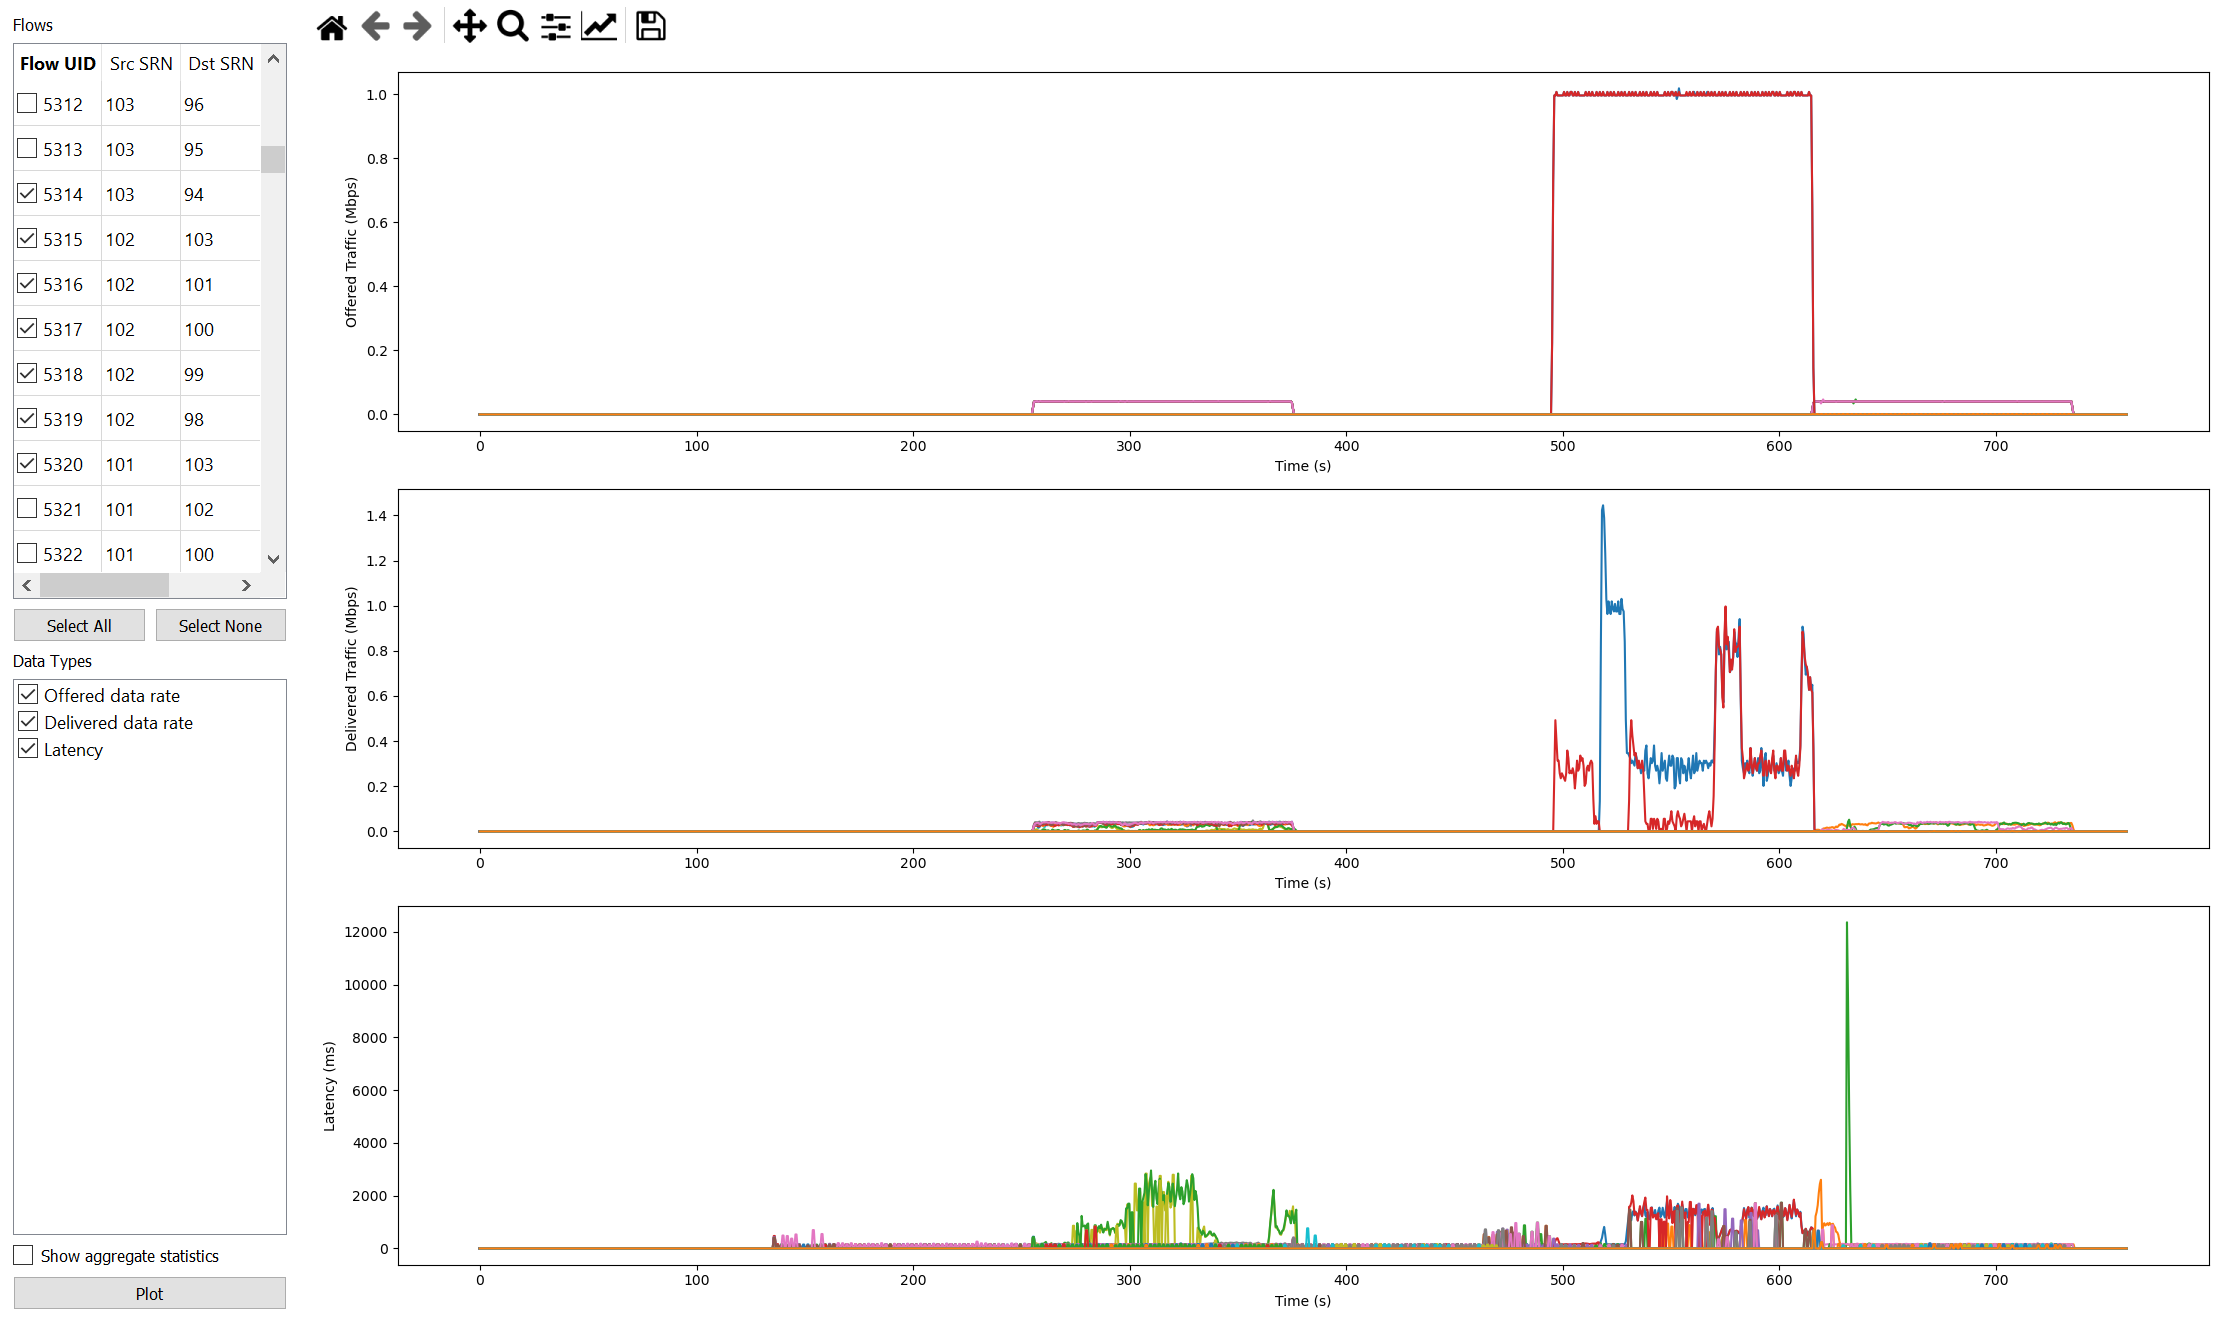
\includegraphics[width = 1.0\textwidth]{Wildfire_NET_2.PNG}}
    \caption{The offered and delivered traffic corresponding to various (selected) links during the Wildfire scenario emulation (Stage $5$)}
    \label{fig:B.15}
\end{figure}

Figs. \ref{fig:B.14} and Fig. \ref{fig:B.15} illustrate the offered traffic corresponding to the individual selected flows, their corresponding delivered traffic, and the latency experienced by these flows as they are being scheduled/delivered by our network, with respect to Stage $1$ and Stage $5$ of the scenario emulation, respectively. Note here that our network is able to deliver almost all of these flows with minimal latency.
\begin{figure} [htb]
    \centerline{
    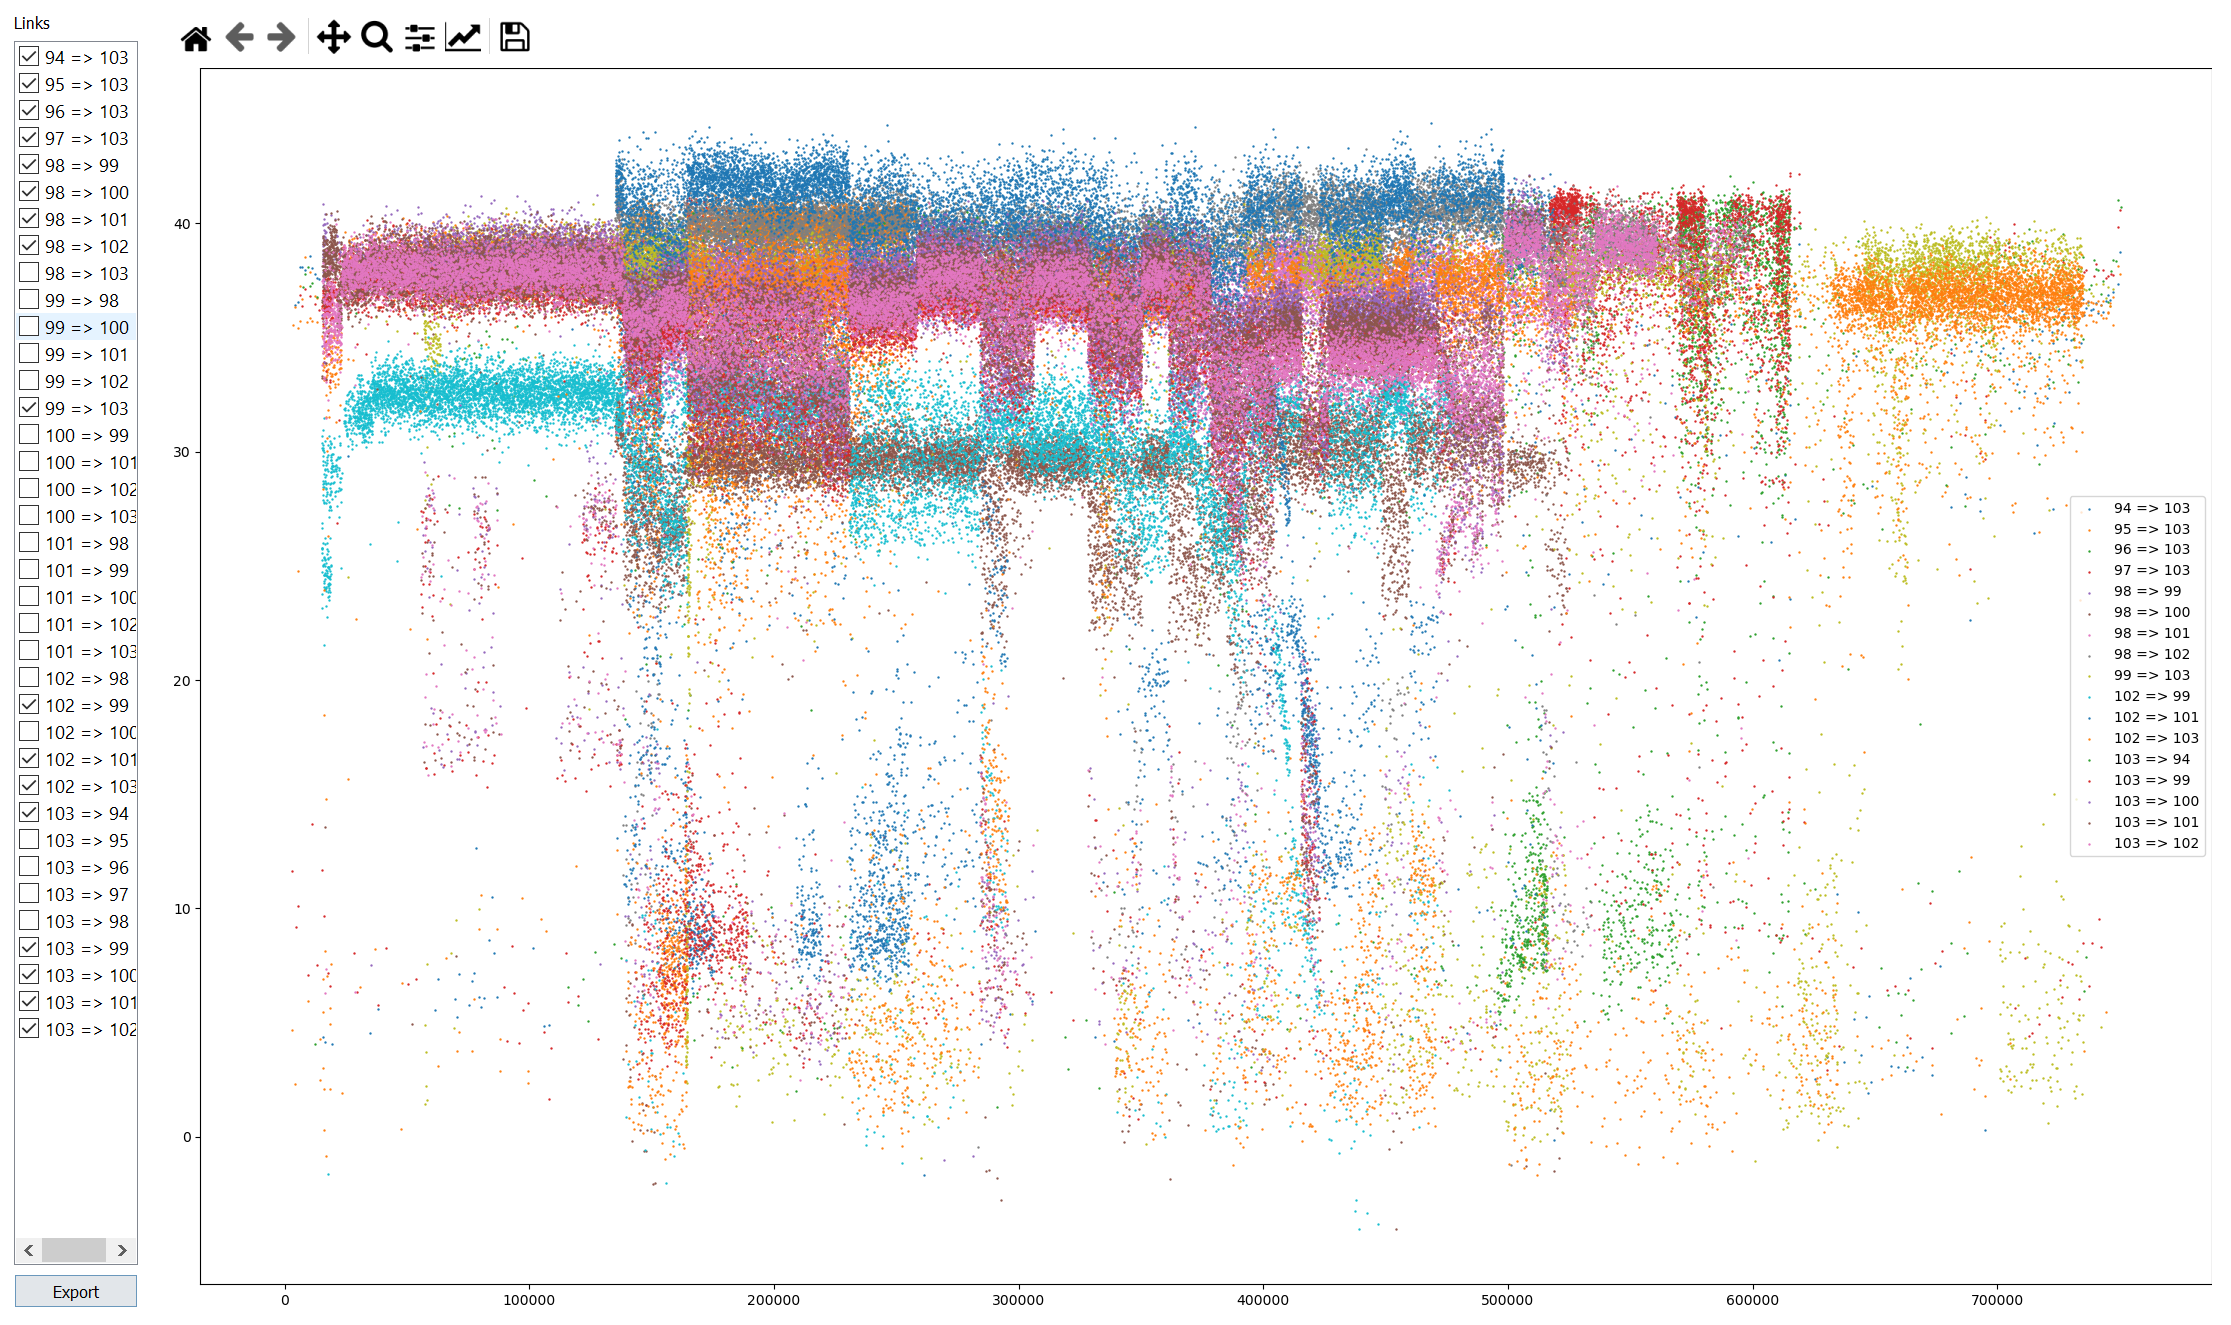
\includegraphics[width = 1.0\textwidth]{Wildfire_SNR.PNG}}
    \caption{The estimated SNR on various (selected links) during the Wildfire scenario emulation}
    \label{fig:B.16}
\end{figure}
\begin{figure} [htb]
    \centerline{
    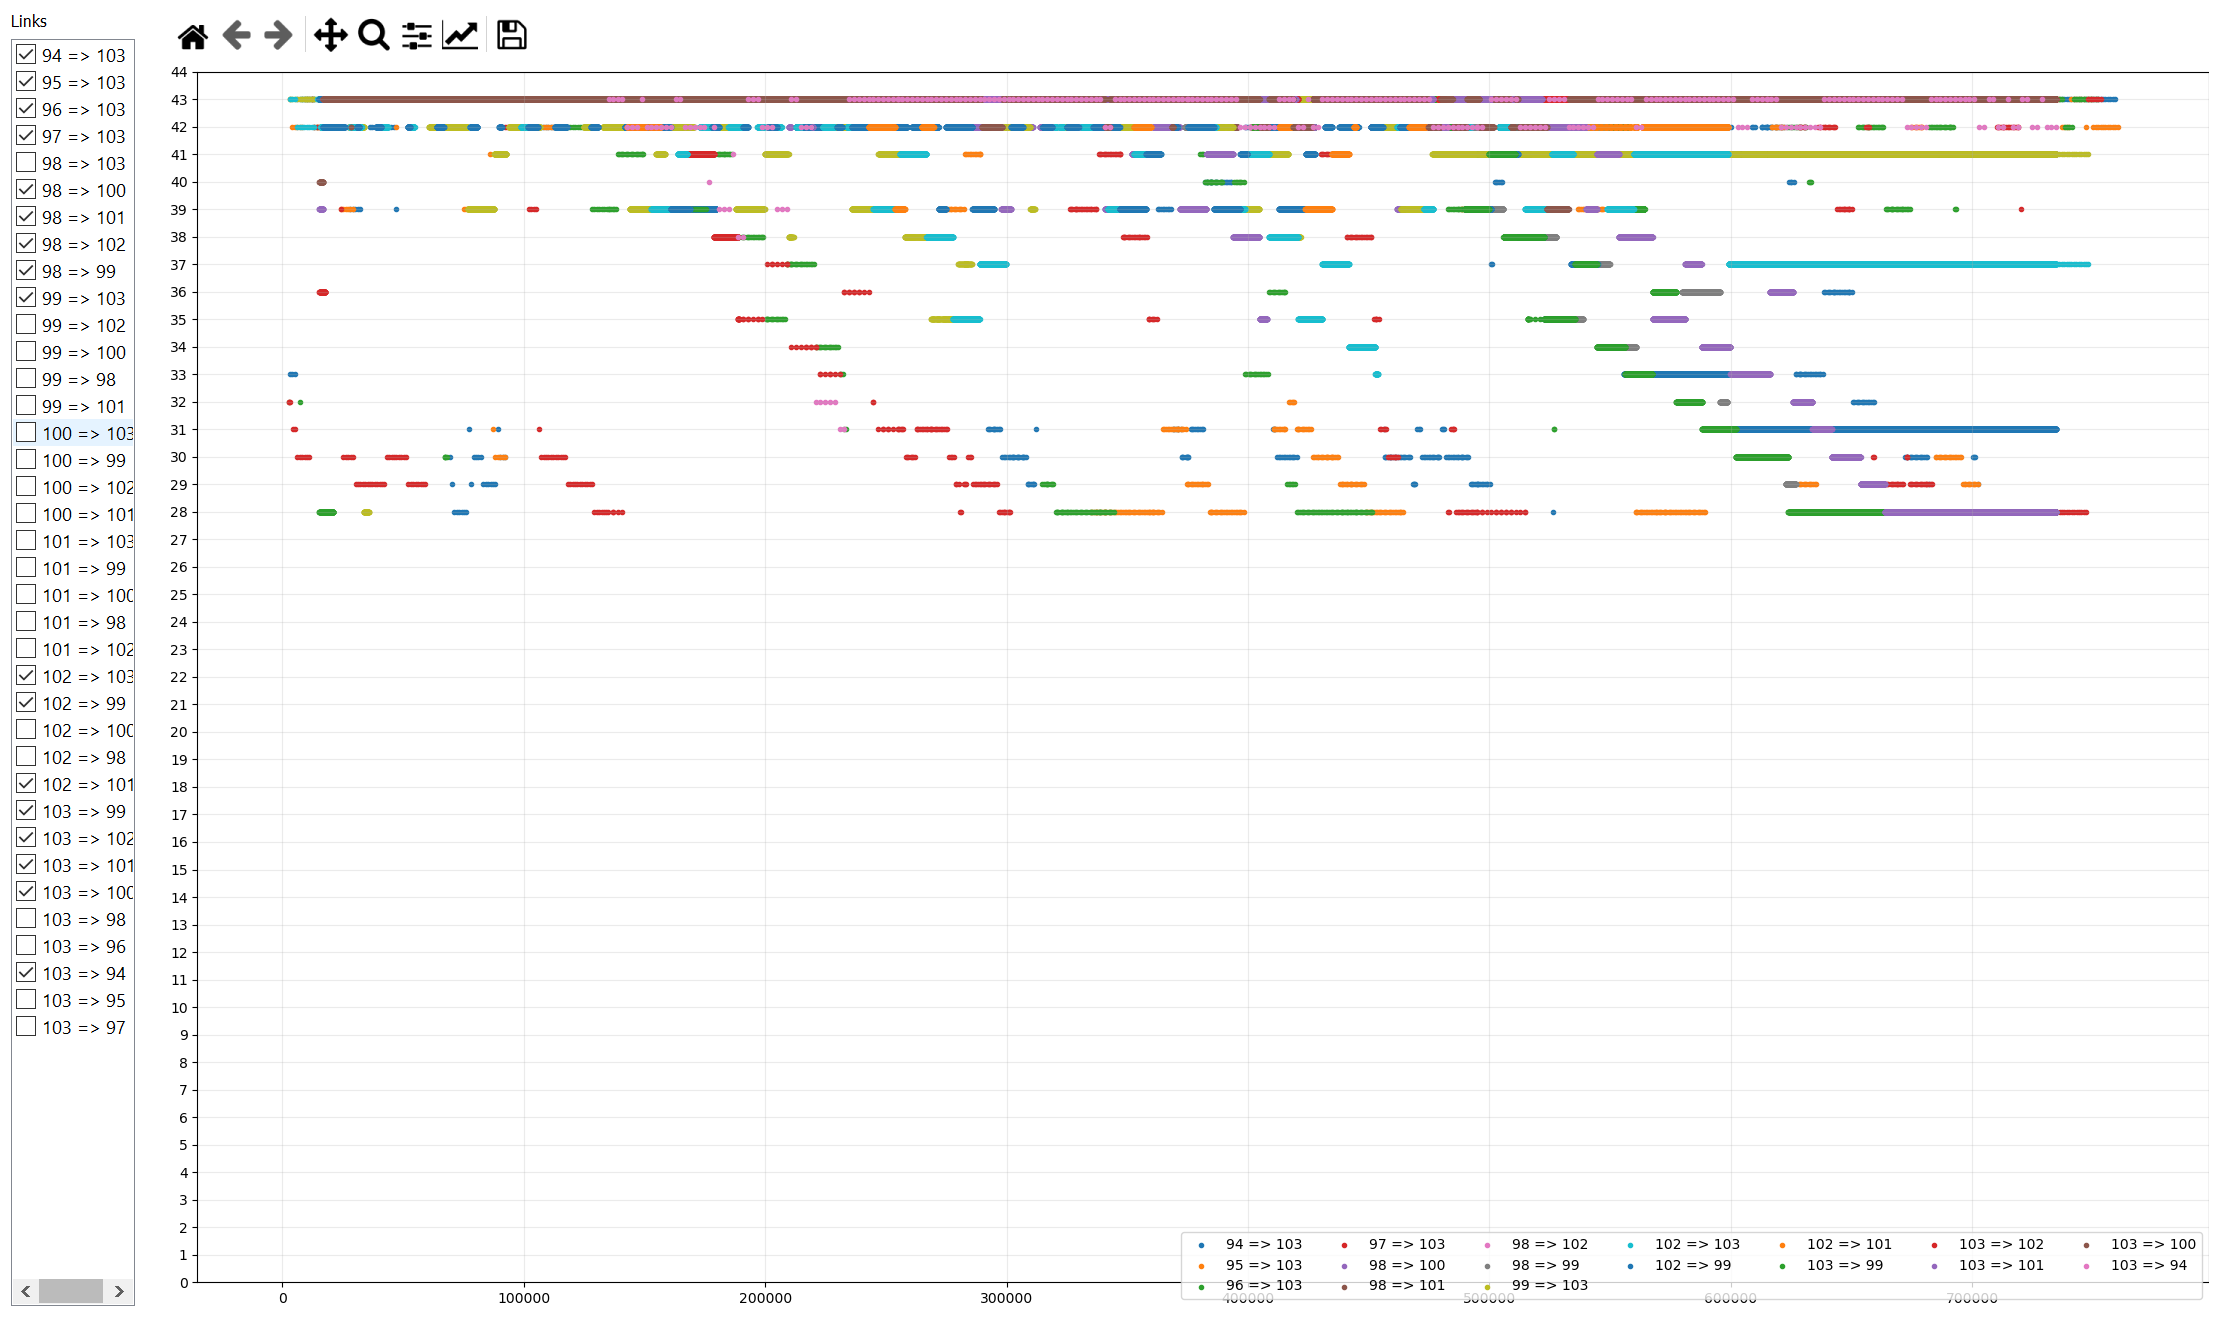
\includegraphics[width = 1.0\textwidth]{Wildfire_MCS.PNG}}
    \caption{The MCS adaptation scheme at each (selected) link during the Wildfire scenario emulation}
    \label{fig:B.17}
\end{figure}

Fig. \ref{fig:B.16} depicts the estimated SNR on various selected links (source SRN - destination SRN), during the progression of the Wildfire scenario\texttt{-{}-}these SNR estimates at each link are, as discussed earlier, employed in the MCS adaptation scheme, the prioritized flow scheduler, and the bandwidth allocation algorithm. Consequently, Fig. \ref{fig:B.17} depicts the MCS adaptation scheme at each of these selected links, adapting to the changing estimated SNR with respect to the corresponding channels used by these links\texttt{-{}-}the Y-axis of the MCS adaptation plot in Fig. \ref{fig:B.17} refers to the C${++}$ enumeration value corresponding to the $(\mathcal{M},\mathcal{R})$ pair, i.e., for example, $43$ in the plot refers to QAM$64$ modulation with a code rate of $\frac{5}{6}$, while $28$ refers to QPSK modulation with $\frac{1}{2}$ code rate\texttt{-{}-}in other words, the highest modulation order used in this Wildfire run is $\mathcal{M}{=}64$ (i.e., QAM$64$), while the lowest modulation order used in $\mathcal{M}{=}4$ (i.e., QPSK).
\begin{figure} [htb]
    \centerline{
    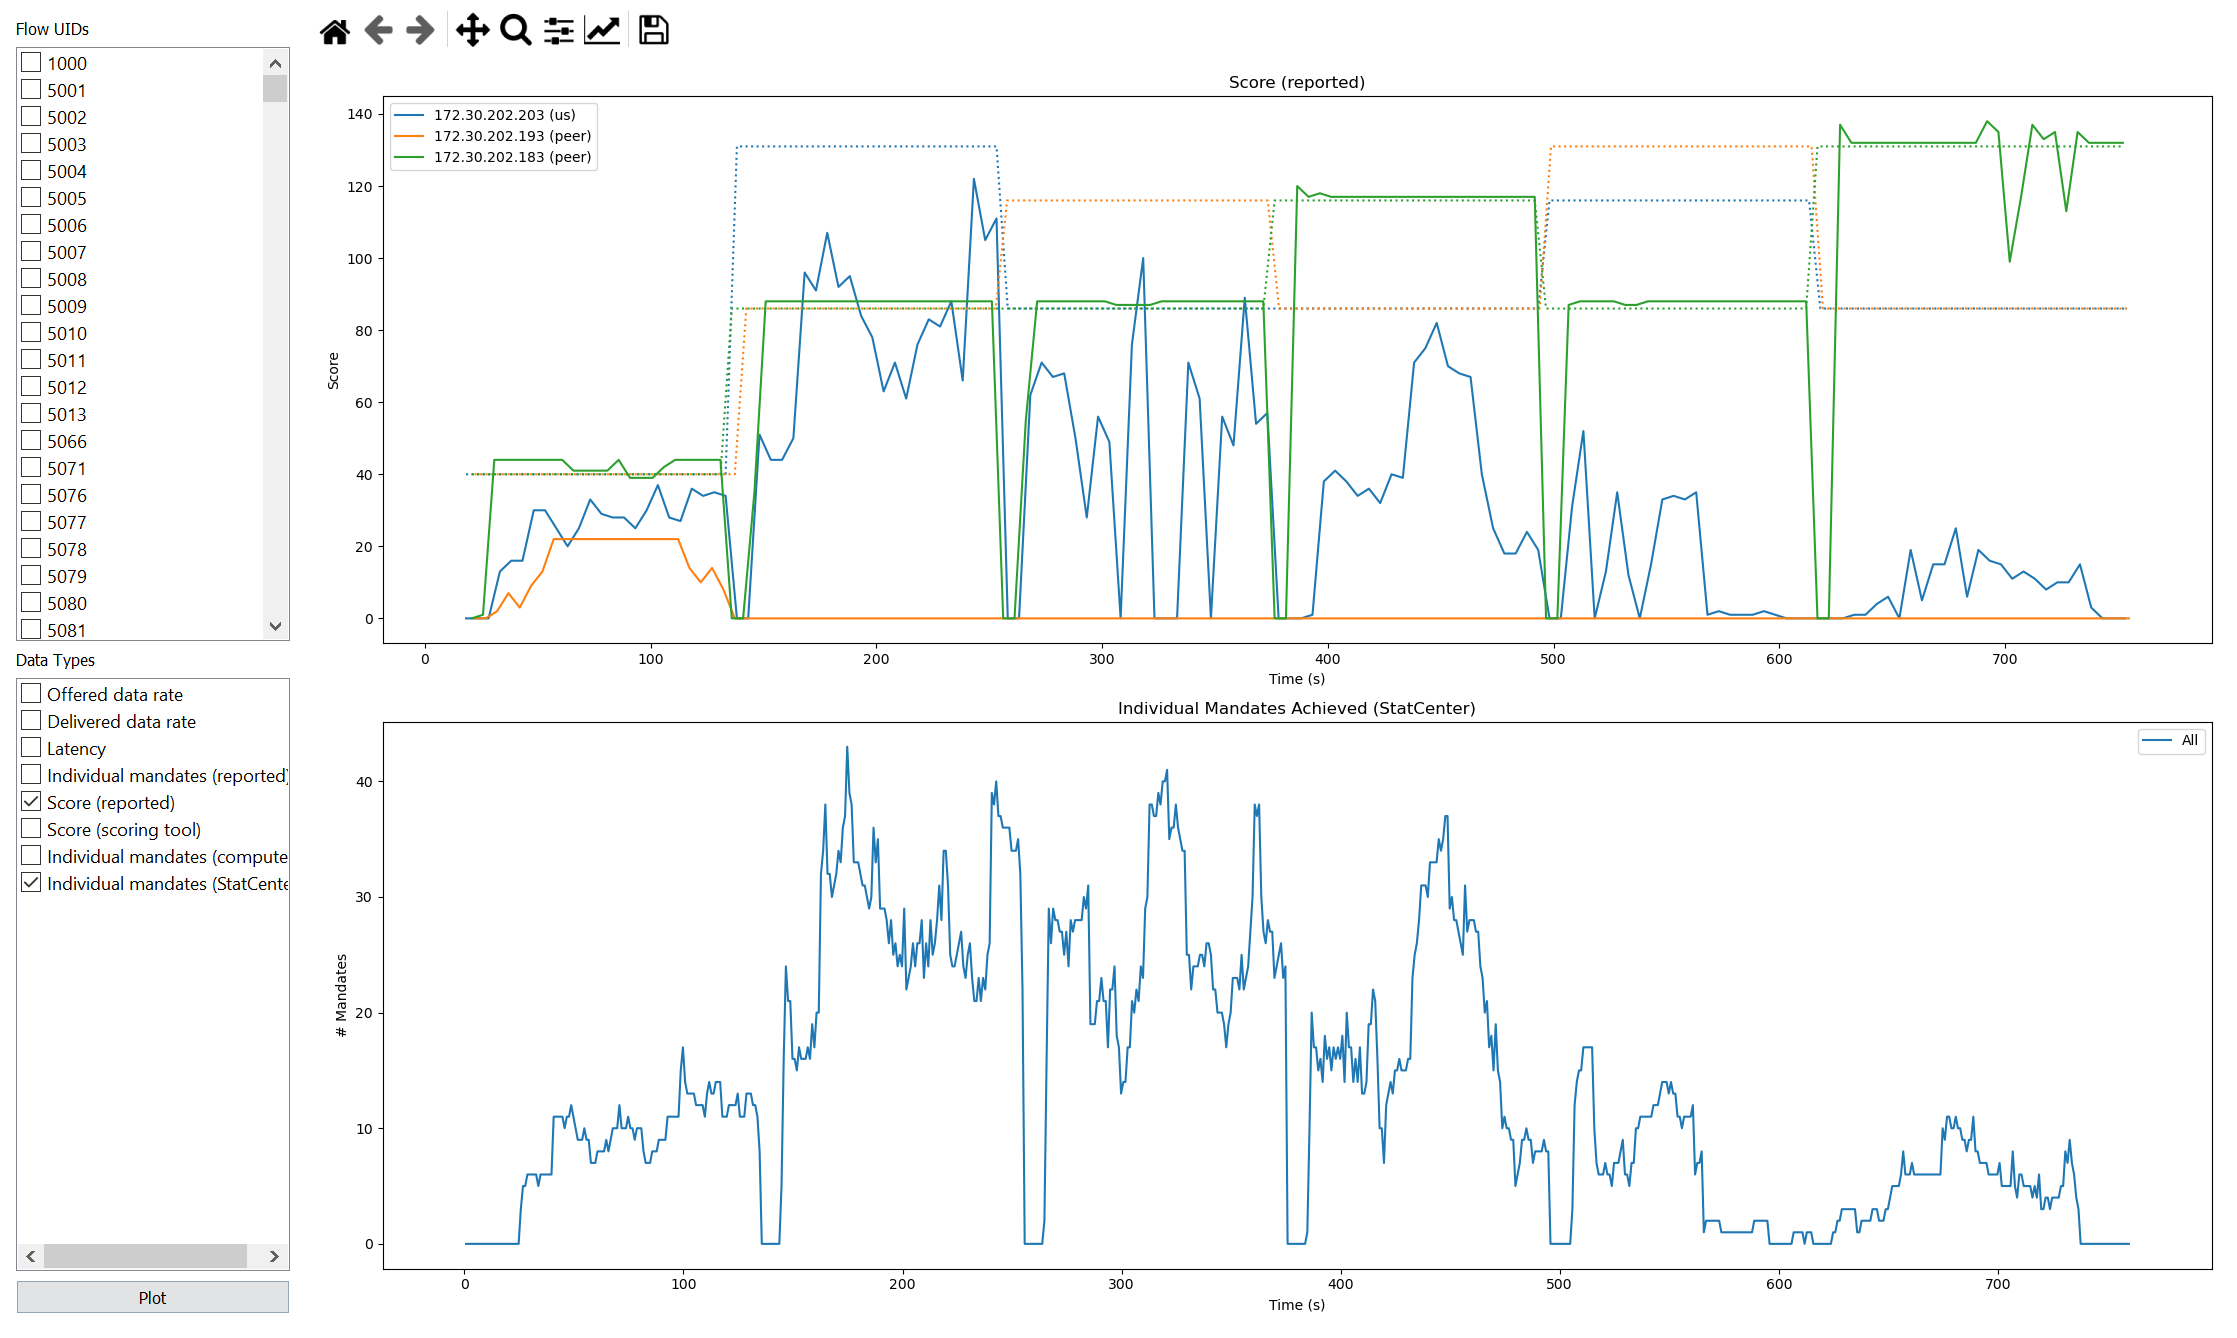
\includegraphics[width = 1.0\textwidth]{Wildfire_Scoring.PNG}}
    \caption{The scores attained by our network and other competing networks during the Wildfire scenario emulation, in addition to the number of QoS mandates satisfied by our network in a given time snapshot}
    \label{fig:B.18}
\end{figure}

Fig. \ref{fig:B.18} illustrates the score obtained by our network (indicated by our Gateway SRN's IP address) along with the scores obtained by our peers (indicated by the IP addresses of their corresponding gateway SRNs) in the scenario emulation. The dotted lines in the first sub-plot indicate the score thresholds that need to be achieved by each network, in a Stage. The second sub-plot illustrates the number of flow-specific QoS mandates that were achieved by our network in a given time snapshot. As evident from the figure, our peer with IP address identifier $172.30.202.183$ performs better than our network, while the other peer with IP address identifier $172.30.202.193$ performs poorly throughout the scenario emulation. Note here that, our network performs quite well in Stages $1$, $2$, and $3$, with our scores above the performance threshold most of time during these initial $3$ stages\texttt{-{}-}however, in Stages $4$, $5$, and $6$, frequent MCS pair switching (adaptation and re-adaptation) as seen in Fig. \ref{fig:B.17}, possibly triggered by poor link quality at a significant number of SRNs (possibly due to aggressive interference from competitor SRNs\texttt{-{}-}specifically, the SRNs from CIRN $172.30.202.183$), causes our performance to deteriorate significantly\texttt{-}leading to scores below the threshold in these stages.
\begin{figure} [htb]
    \centerline{
    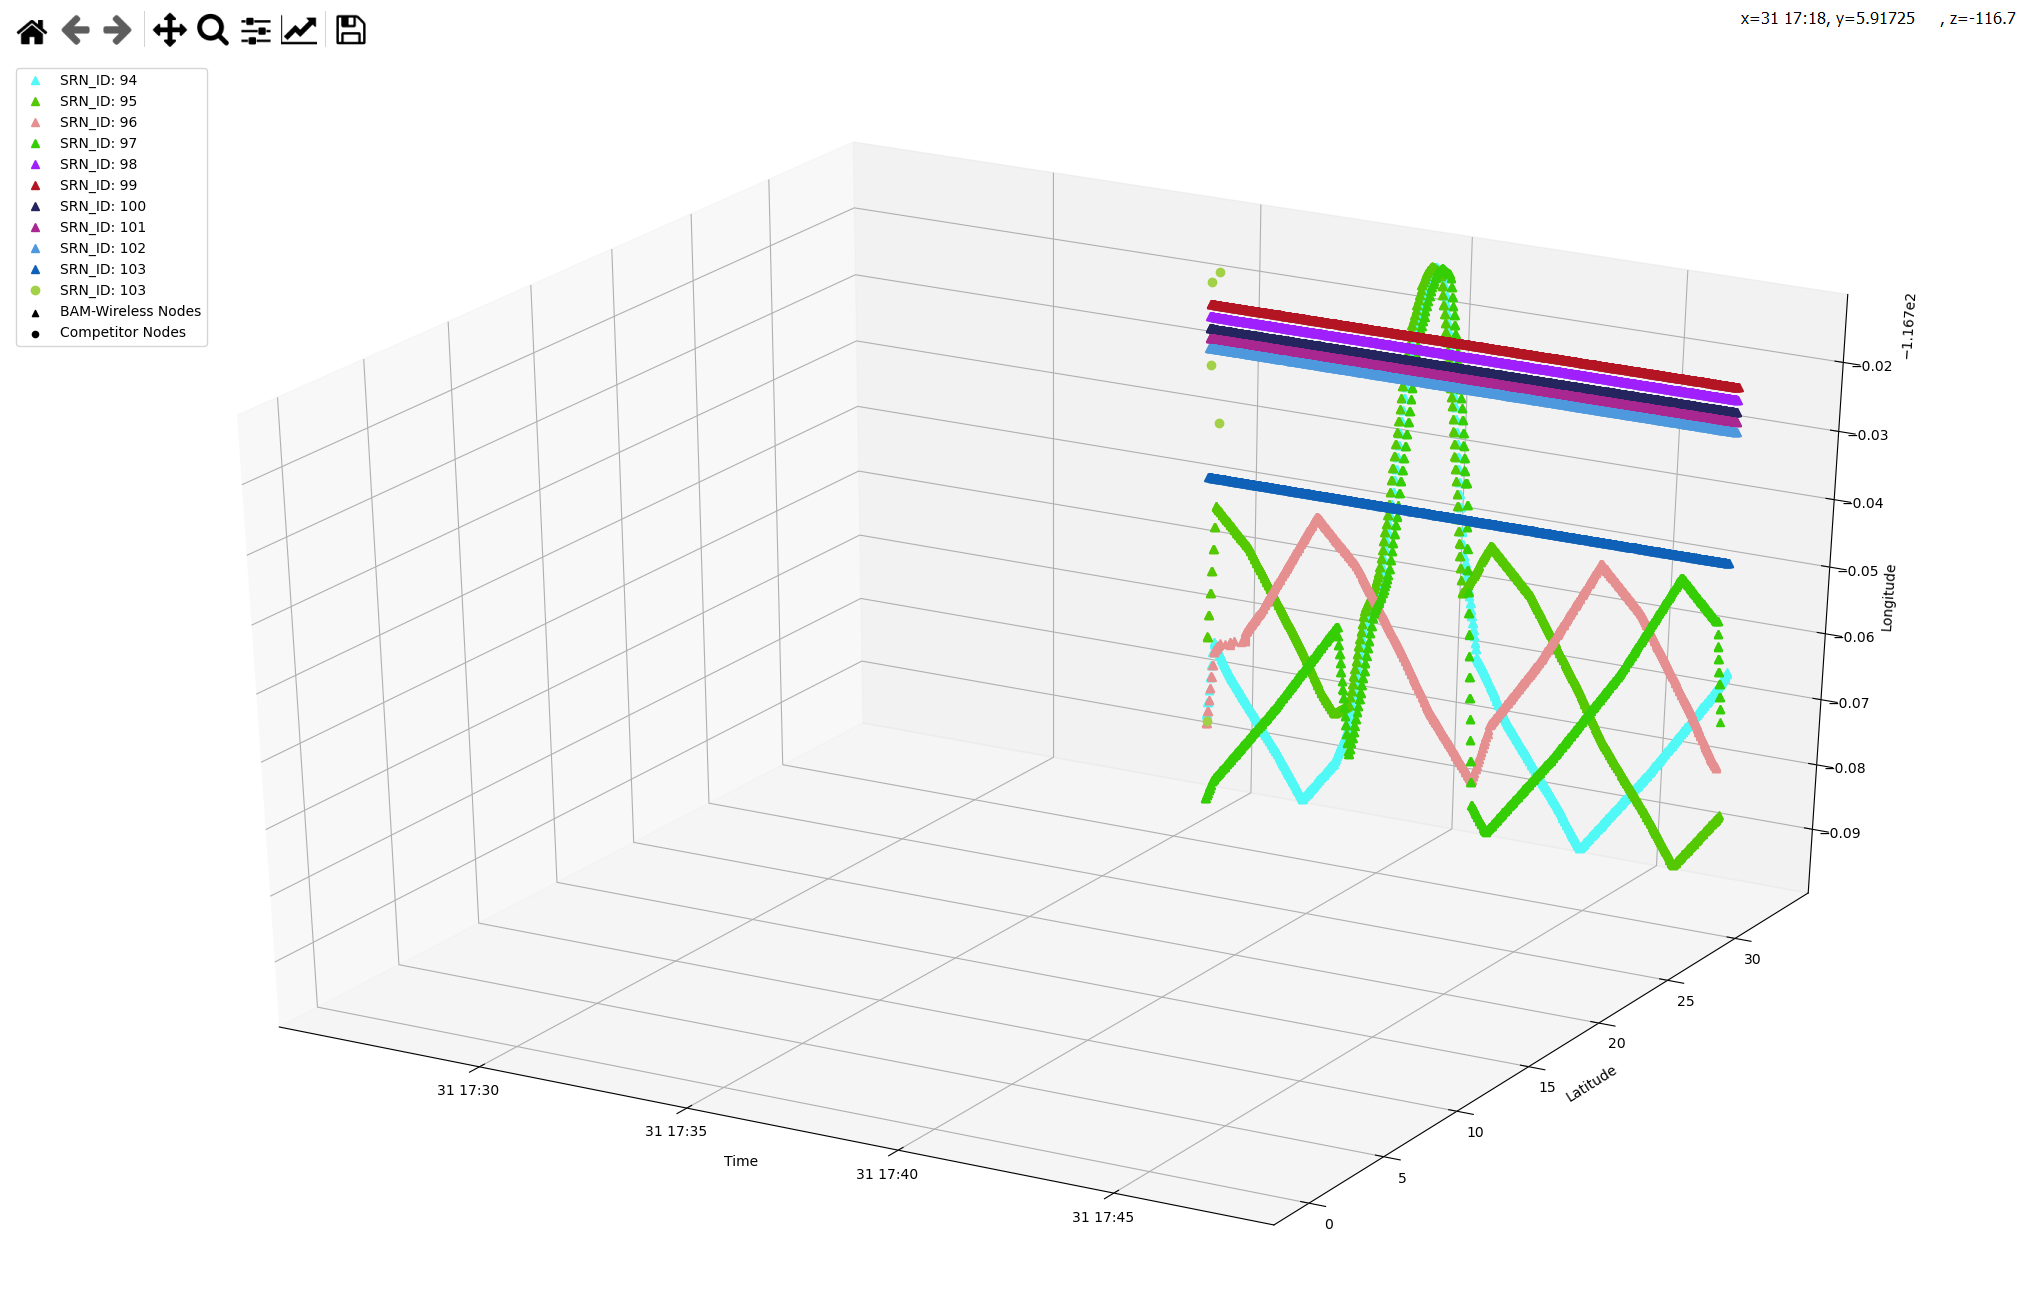
\includegraphics[width = 1.0\textwidth]{Wildfire_GPS.PNG}}
    \caption{The reported GPS locations of our SRNs, in addition to those of our competing SRNs, during the Wildfire scenario emulation}
    \label{fig:B.19}
\end{figure}
\begin{figure} [htb]
    \centerline{
    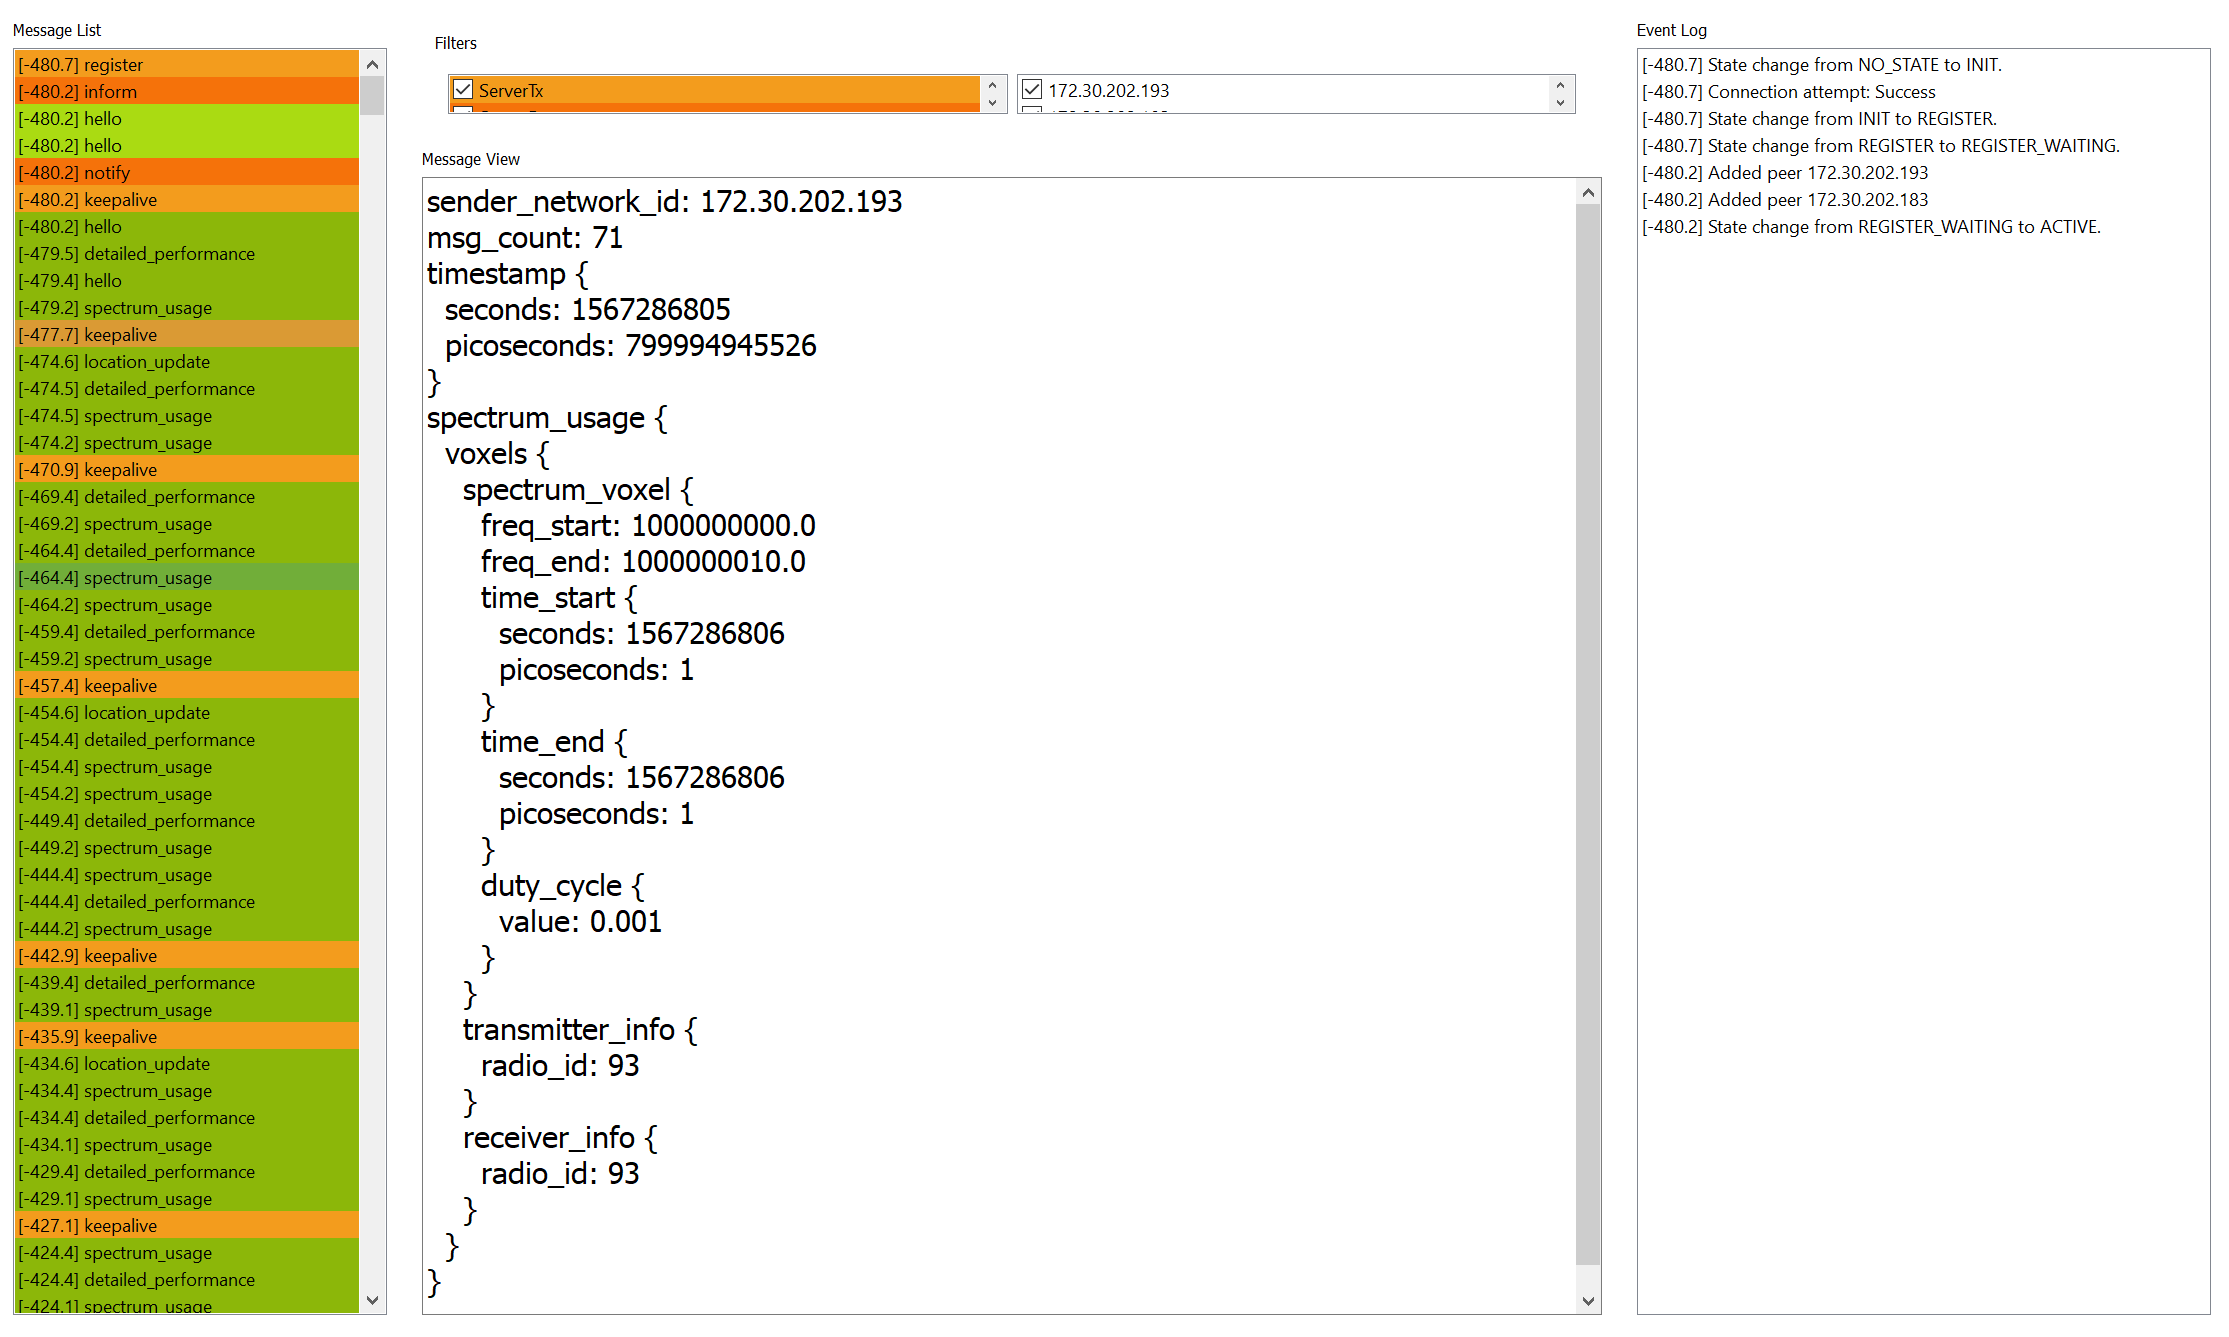
\includegraphics[width = 0.8\textwidth]{Wildfire_Collab.PNG}}
    \caption{The description of various CIL message exchanges between our network and the collaboration server, in addition to those between our network and our peers, during the Wildfire scenario emulation}
    \label{fig:B.20}
\end{figure}
\begin{figure} [htb]
    \centerline{
    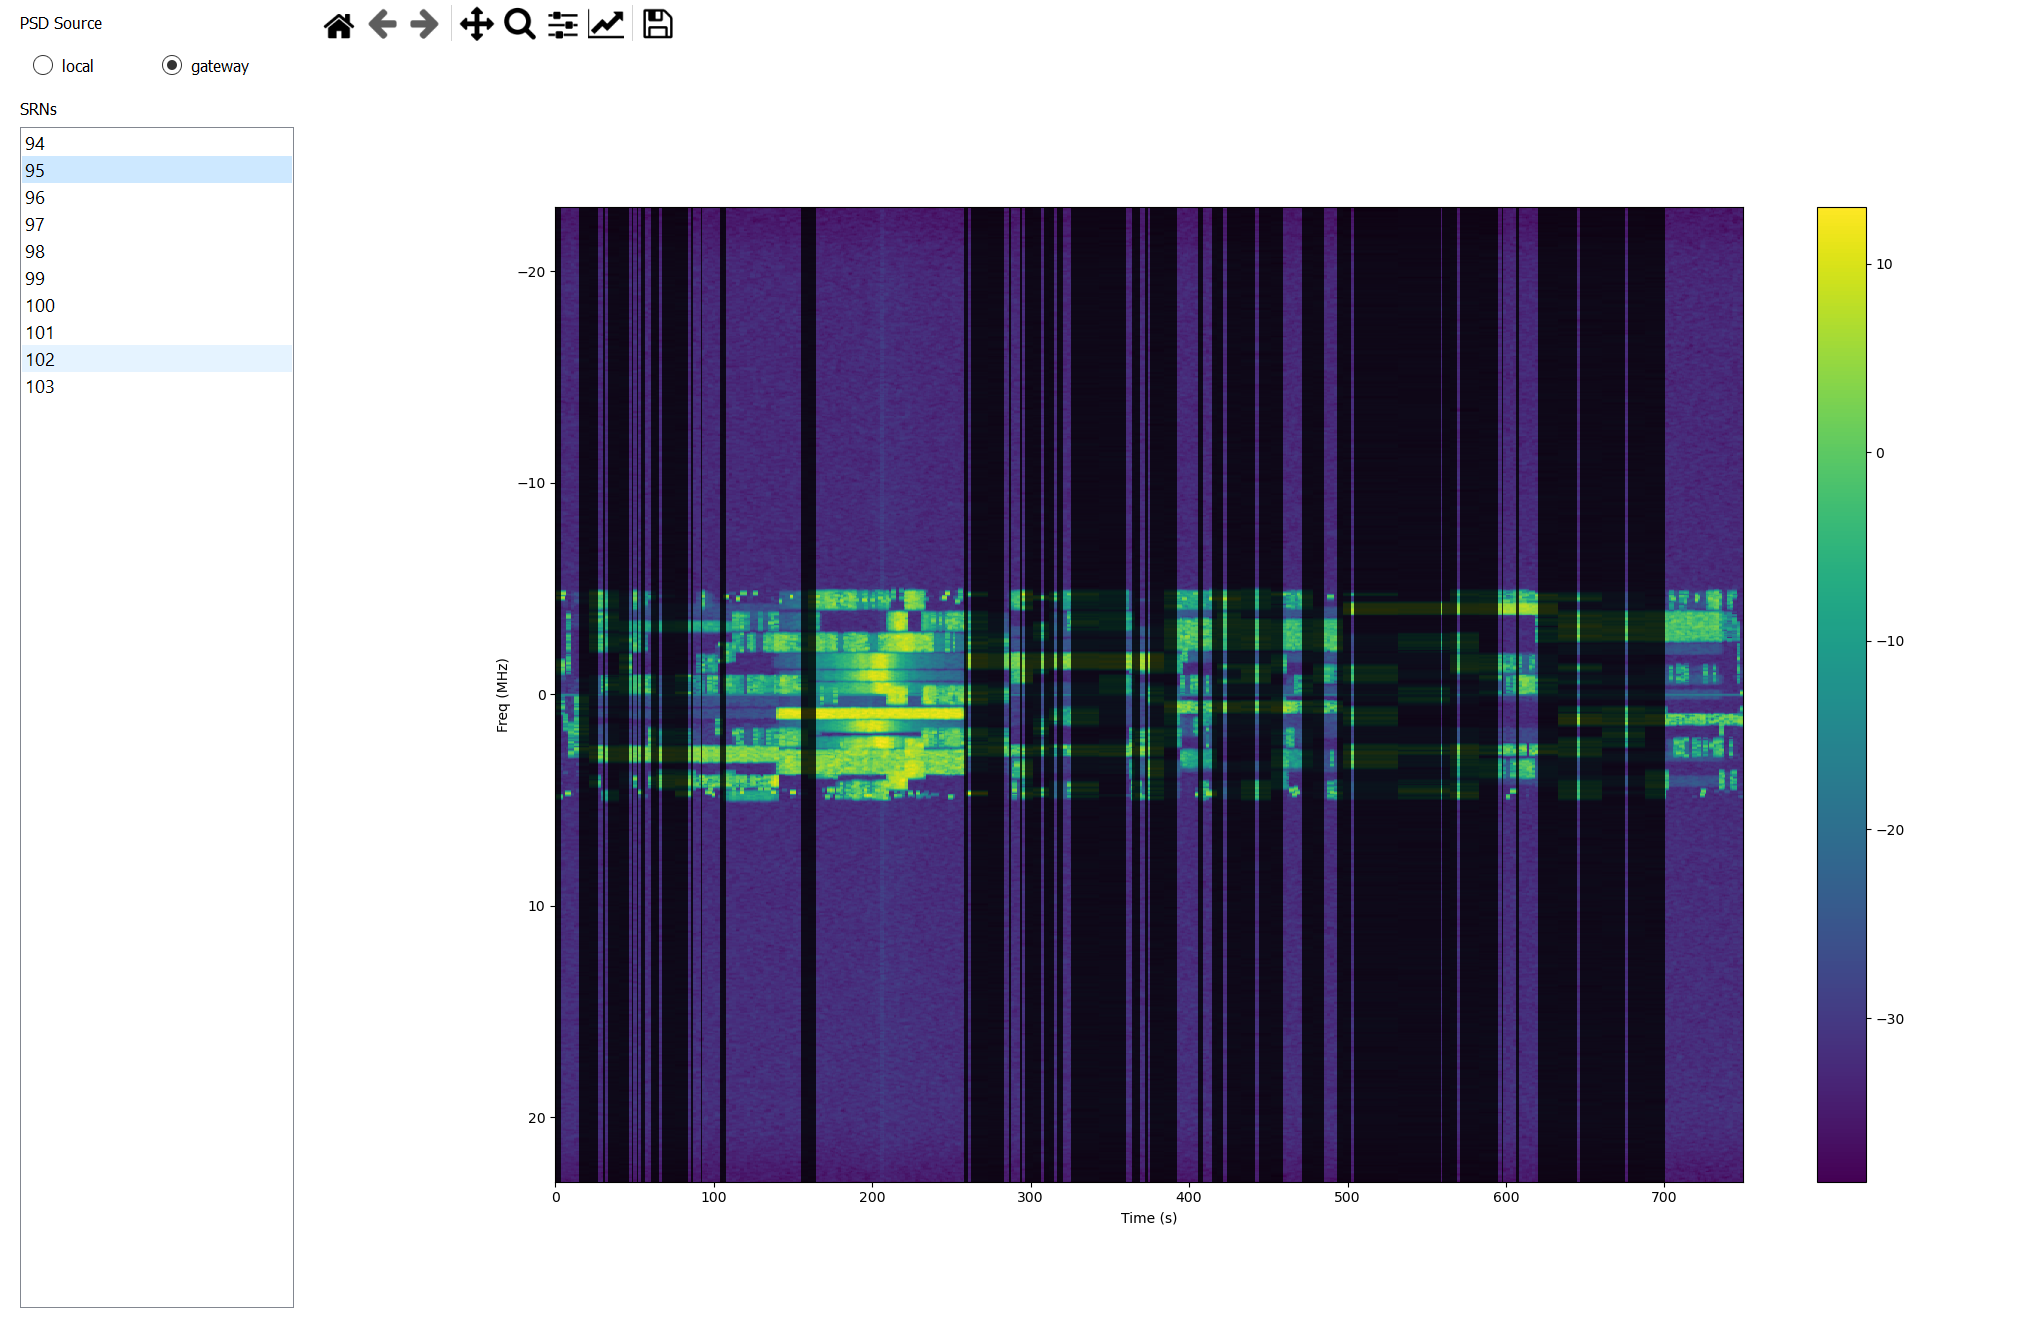
\includegraphics[width = 0.8\textwidth]{Wildfire_PSD.PNG}}
    \caption{The PSD measurements received at our Gateway SRN from one particular SRN in our network (selected), in order to obtain location-specific spectrum occupancy information, during the Wildfire scenario emulation}
    \label{fig:B.21}
\end{figure}

The reported GPS locations (latitude, longitude) of the SRNs in our CIRN, and the SRNs in our competitors' CIRNs, over time, are depicted in a $3$-dimensional time plot shown in Fig. \ref{fig:B.19}. The location information of these SRNs\texttt{-{}-}particularly, in relation to physical obstacles (emulated) and competitor SRNs, is employed in the channel allocation algorithm in our Gateway SRN. Fig. \ref{fig:B.20} illustrates the various timestamped CIL messages (both Client-Server messages and Peer-to-Peer messages) received by our Gateway SRN over the collaboration network\texttt{-{}-}these messages are exploited by our Gateway SRN, which along with the collated location-specific PSD measurements: one such PSD measurement in a given time snapshot observed at SRN with ID\texttt{-}$95$ and sent to our Gateway, is depicted in Fig. \ref{fig:B.21}\texttt{-{}-}determines a channel allocation (center frequencies) that minimizes the total interference caused at our SRNs by our competitors. Consequently, from an overall scenario duration perspective, the channel allocations of our network are collated into one ``big-picture" illustration, shown in Fig. \ref{fig:B.22}\texttt{-{}-}it is evident from this figure (the plot and the table underneath it) that the channel and bandwidth allocation strategy of our network is pretty consistent and stable throughout the scenario emulation.
\begin{figure} [htb]
    \centerline{
    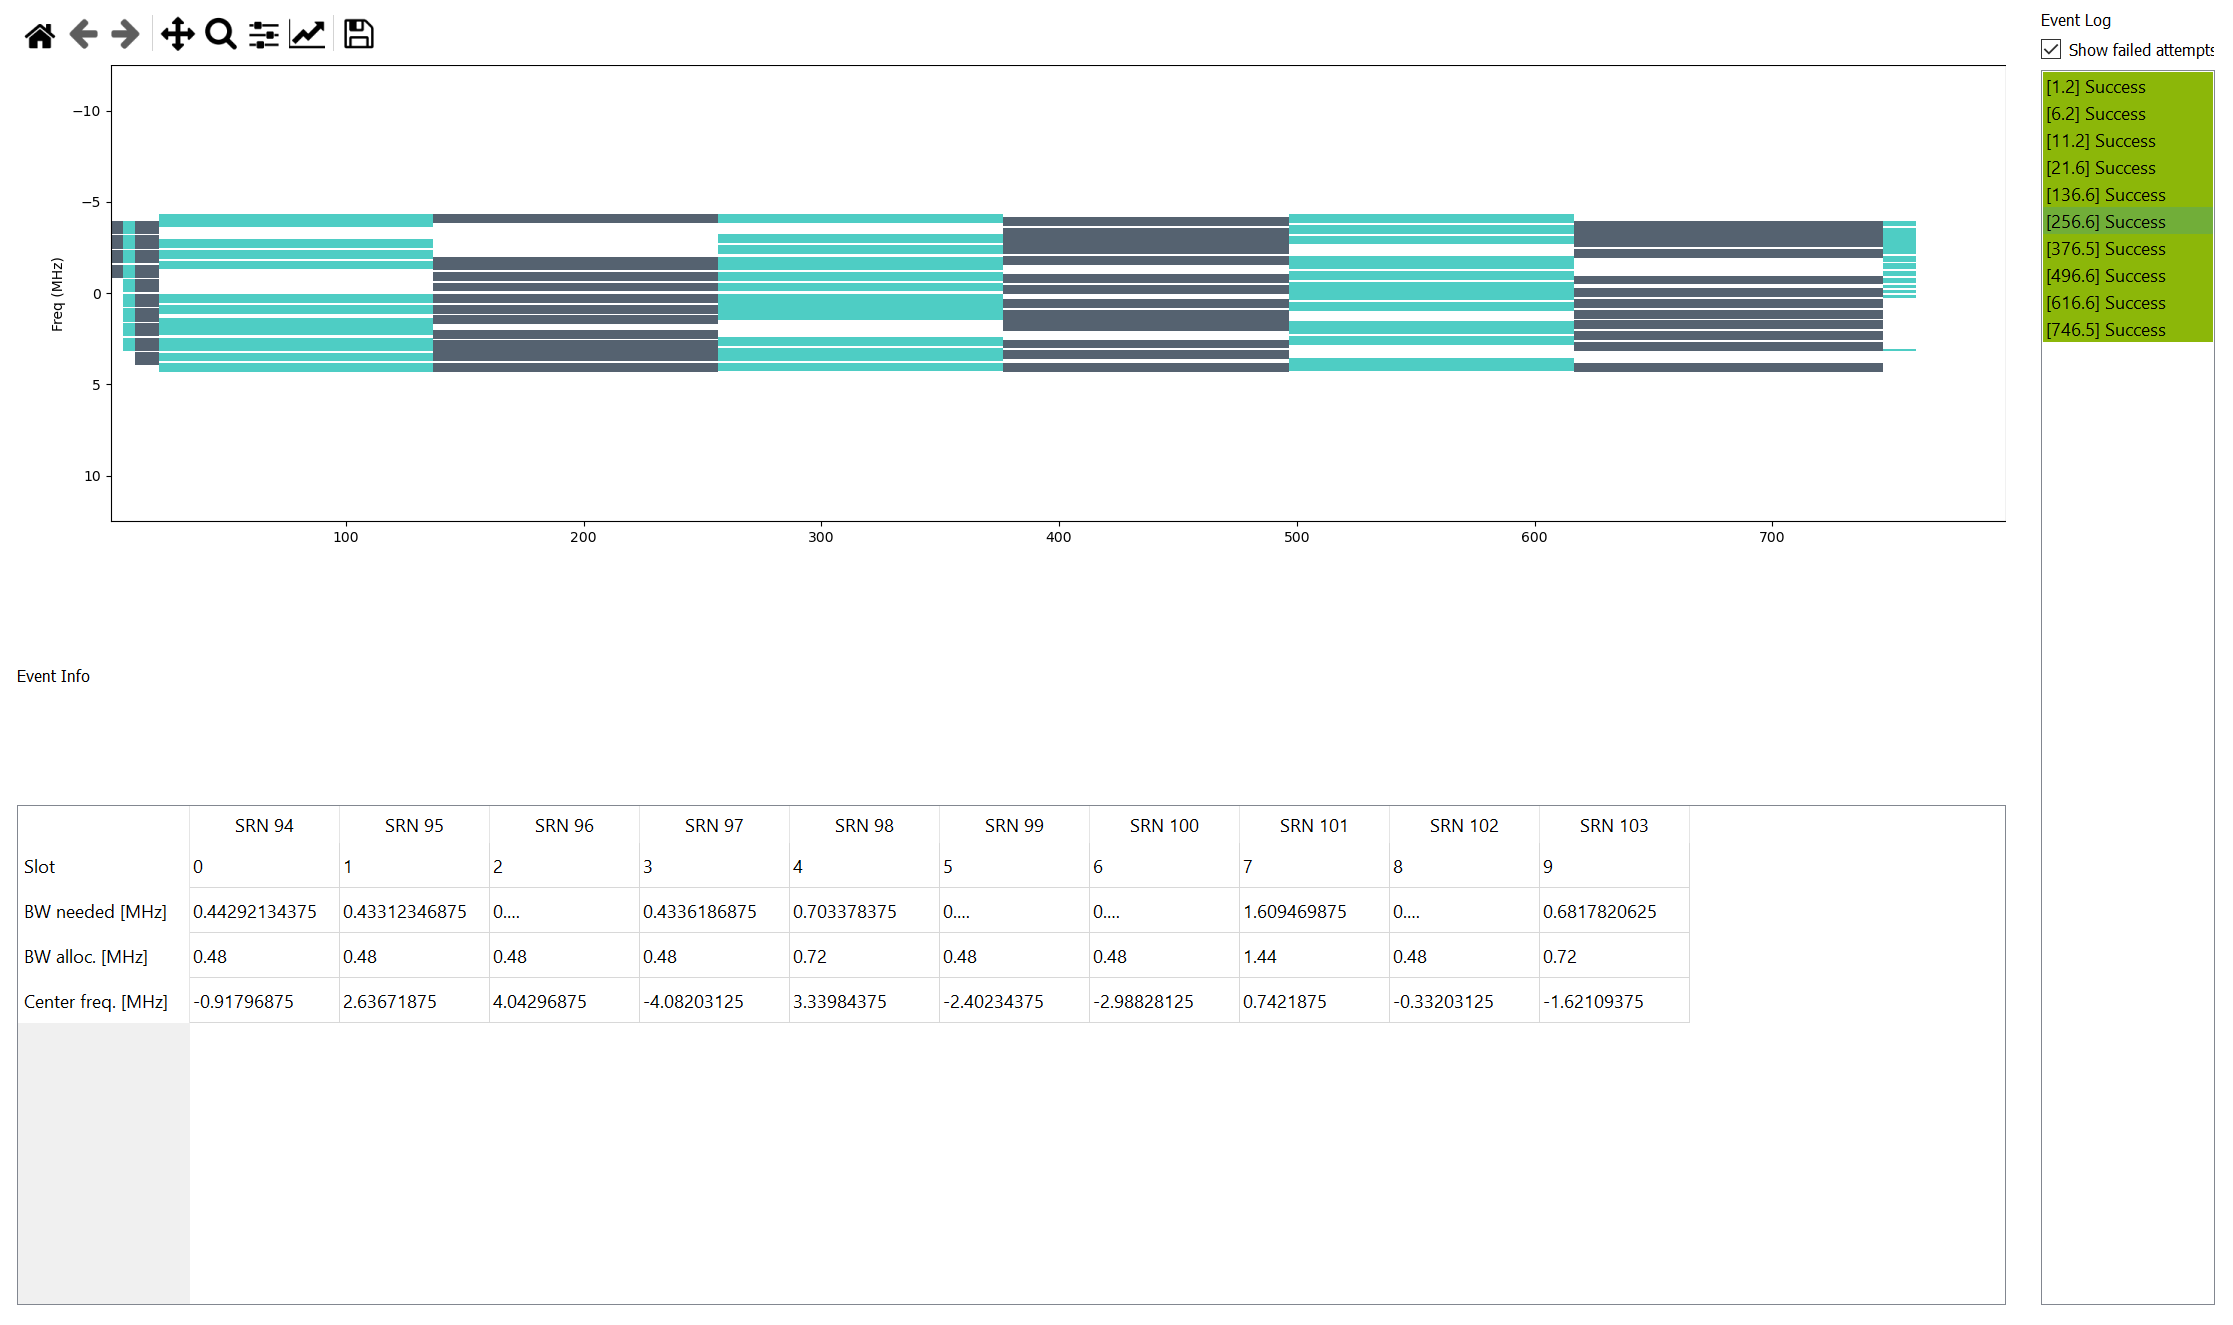
\includegraphics[width = 1.0\textwidth]{Wildfire_Channel_Alloc.PNG}}
    \caption{The spectrum occupancy behavior of SRNs in our network (as guided by our Gateway SRN) during the Wildfire scenario emulation}
    \label{fig:B.22}
\end{figure}
\section{Conclusion}\label{B.V}
In this chapter, we discussed the design principles of our cognitive radio developed for the DARPA SC2 Grand Challenge\texttt{-{}-}the transmission power control algorithm in the PHY for incumbent protection, the robust FSK control channel design, the high data rate DFT spread OFDM link for data traffic and ``long" control messages, the MCS adaptation algorithm in the PHY, the prioritized value-per-resource flow scheduling heuristic in the DLL with recursive revisitation, the channel and bandwidth allocation heuristic in the MAC, and the Dijkstra algorithm based multi-hop routing heuristic in the NET; the Radio Command and Control API (C2API) of the Colosseum that facilitates network management and orchestration; and the CIRN Interface Language (CIL) specifications, along with details about the collaboration network. Additionally, we presented component-wise plots illustrating the operational capabilities of our radios\texttt{-{}-}driven by the underlying design principles mentioned earlier, and evaluation of our network's performance against that of our competitors (other teams in this Grand Challenge: Northeastern University, Vanderbilt University, University of Florida, Virginia Tech (with Lockheed Martin), and Rutgers University, to name a few) in a military deployment scenario, i.e., Alleys of Austin, and a disaster-relief deployment scenario, i.e., Wildfire. Having presented the design of a cognitive radio node (and its deployment in a network of peers) and analyzed the operational capabilities and performance of our radios in quasi-collaborative scenario emulations, we now narrow our focus down to a specific problem\texttt{-{}-}the spectrum sensing and access problem in the MAC layer, and instead of proposing a complex heuristic like we did in this chapter, in the next chapter, we detail a highly rigorous approach to solve for the optimal spectrum sensing and access policy using an POMDP formulation.